\documentclass[a4paper,11pt]{book}
%\documentclass[a4paper,twoside,11pt,titlepage]{book}
\usepackage{listings}
\usepackage[utf8]{inputenc}
\usepackage[spanish]{babel}

% \usepackage[style=list, number=none]{glossary} %
%\usepackage{titlesec}
%\usepackage{pailatino}

\decimalpoint
\usepackage{dcolumn}
\newcolumntype{.}{D{.}{\esperiod}{-1}}
\makeatletter
\addto\shorthandsspanish{\let\esperiod\es@period@code}
\makeatother


%\usepackage[chapter]{algorithm}
\RequirePackage{verbatim}
%\RequirePackage[Glenn]{fncychap}
\usepackage{fancyhdr}
\usepackage{graphicx}
\usepackage{afterpage}
\usepackage{enumerate}
\usepackage{enumitem}
\usepackage{longtable}
\usepackage{xcolor}
\usepackage{algpseudocode}
\usepackage{algorithm}
\usepackage[pdfborder={000}]{hyperref} %referencia
\usepackage{amsmath}

% ********************************************************************
% Re-usable information
% ********************************************************************
\newcommand{\myTitle}{Desarrollo de un motor gráfico utilizando Vulkan\xspace}
\newcommand{\myDegree}{Grado en Ingeniería Informática\xspace}
\newcommand{\myName}{Jose Luis Martínez Ortiz\xspace}
\newcommand{\myProf}{Alejandro José León Salas\xspace}
\newcommand{\myOtherProf}{\xspace}
%\newcommand{\mySupervisor}{Put name here\xspace}
\newcommand{\myFaculty}{Escuela Técnica Superior de Ingenierías Informática y de
Telecomunicación\xspace}
\newcommand{\myFacultyShort}{E.T.S. de Ingenierías Informática y de
Telecomunicación\xspace}
\newcommand{\myDepartment}{Departamento de Lenguajes y Sistemas Informáticas\xspace}
\newcommand{\myUni}{\protect{Universidad de Granada}\xspace}
\newcommand{\myLocation}{Granada\xspace}
\newcommand{\myTime}{\today\xspace}
\newcommand{\myVersion}{Version 0.1\xspace}


\hypersetup{
pdfauthor = {\myName (joselmo@correo.ugr.es)},
pdftitle = {\myTitle},
pdfsubject = {},
pdfkeywords = {OpenGl, Modelador, Geometry Processing, ...},
pdfcreator = {LaTeX con el paquete ....},
pdfproducer = {pdflatex}
}

%\hyphenation{}


%\usepackage{doxygen/doxygen}
%\usepackage{pdfpages}
\usepackage{url}
\usepackage{colortbl,longtable}
\usepackage[stable]{footmisc}
\usepackage{index}

\makeindex
%\usepackage[style=long, cols=2,border=plain,toc=true,number=none]{glossary}
% \makeglossary

% Definición de comandos que me son tiles:
%\renewcommand{\indexname}{Índice alfabético}
%\renewcommand{\glossaryname}{Glosario}

\pagestyle{fancy}
\fancyhf{}
\fancyhead[LO]{\leftmark}
\fancyhead[RE]{\rightmark}
\fancyhead[RO,LE]{\textbf{\thepage}}
\renewcommand{\chaptermark}[1]{\markboth{\textbf{#1}}{}}
\renewcommand{\sectionmark}[1]{\markright{\textbf{\thesection. #1}}}

\setlength{\headheight}{1.5\headheight}

\newcommand{\HRule}{\rule{\linewidth}{0.5mm}}
%Definimos los tipos teorema, ejemplo y definición podremos usar estos tipos
%simplemente poniendo \begin{teorema} \end{teorema} ...
\newtheorem{teorema}{Teorema}[chapter]
\newtheorem{ejemplo}{Ejemplo}[chapter]
\newtheorem{definicion}{Definición}[chapter]

\definecolor{gray97}{gray}{.97}
\definecolor{gray75}{gray}{.75}
\definecolor{gray45}{gray}{.45}
\definecolor{gray30}{gray}{.94}

\lstset{ frame=Ltb,
     framerule=0.5pt,
     aboveskip=0.5cm,
     framextopmargin=3pt,
     framexbottommargin=3pt,
     framexleftmargin=0.1cm,
     framesep=0pt,
     rulesep=.4pt,
     backgroundcolor=\color{gray97},
     rulesepcolor=\color{black},
     %
     stringstyle=\ttfamily,
     showstringspaces = false,
     basicstyle=\scriptsize\ttfamily,
     commentstyle=\color{gray45},
     keywordstyle=\bfseries,
     %
     numbers=left,
     numbersep=6pt,
     numberstyle=\tiny,
     numberfirstline = false,
     breaklines=true,
   }
 
% minimizar fragmentado de listados
\lstnewenvironment{listing}[1][]
   {\lstset{#1}\pagebreak[0]}{\pagebreak[0]}

\lstdefinestyle{CodigoC}
   {
	basicstyle=\scriptsize,
	frame=single,
	language=C,
	numbers=left
   }
\lstdefinestyle{CodigoC++}
   {
	basicstyle=\small,
	frame=single,
	backgroundcolor=\color{gray30},
	language=C++,
	numbers=left
   }

 
\lstdefinestyle{Consola}
   {basicstyle=\scriptsize\bf\ttfamily,
    backgroundcolor=\color{gray30},
    frame=single,
    numbers=none
   }


\newcommand{\bigrule}{\titlerule[0.5mm]}


%Para conseguir que en las páginas en blanco no ponga cabecerass
\makeatletter
\def\clearpage{%
  \ifvmode
    \ifnum \@dbltopnum =\m@ne
      \ifdim \pagetotal <\topskip
        \hbox{}
      \fi
    \fi
  \fi
  \newpage
  \thispagestyle{empty}
  \write\m@ne{}
  \vbox{}
  \penalty -\@Mi
}
\makeatother

\usepackage{pdfpages}
\begin{document}
\begin{titlepage}
 
 
\newlength{\centeroffset}
\setlength{\centeroffset}{-0.5\oddsidemargin}
\addtolength{\centeroffset}{0.5\evensidemargin}
\thispagestyle{empty}

\noindent\hspace*{\centeroffset}\begin{minipage}{\textwidth}

%\centering
%
\includegraphics[width=0.9\textwidth]{imagenes/logo_ugr.jpg}\\[1.4cm]

\textsc{ \Large TRABAJO FIN DE GRADO\\[0.2cm]}
\textsc{ INGENIERÍA EN INFORMÁTICA}\\[1cm]
% Upper part of the page
% 
% Title
{\Huge\bfseries Desarrollo de un motor gráfico utilizando OpenGL/Vulkan\\
}
\noindent\rule[-1ex]{\textwidth}{3pt}\\[3.5ex]
{\large\bfseries }
\end{minipage}

\vspace{2.5cm}
\noindent\hspace*{\centeroffset}\begin{minipage}{\textwidth}
\centering

\textbf{Autor}\\ {Jose Luis Martínez Ortiz}\\[2.5ex]
\textbf{Directores}\\
{Alejandro José León Salas}\\[2cm]

\includegraphics[width=0.3\textwidth]{imagenes/etsiit_logo.png}\\[0.1cm]
\textsc{Escuela Técnica Superior de Ingenierías Informática y de Telecomunicación}\\
\textsc{---}\\
Granada, 6 de Septiembre de 2018
\end{minipage}
%\addtolength{\textwidth}{\centeroffset}
%\vspace{\stretch{2}}
\end{titlepage}



\chapter*{}
%\thispagestyle{empty}
%\cleardoublepage

%\thispagestyle{empty}

\begin{titlepage}
 
 
\setlength{\centeroffset}{-0.5\oddsidemargin}
\addtolength{\centeroffset}{0.5\evensidemargin}
\thispagestyle{empty}

\noindent\hspace*{\centeroffset}\begin{minipage}{\textwidth}

\centering
%
\includegraphics[width=0.9\textwidth]{imagenes/logo_ugr.jpg}\\[1.4cm]

%\textsc{ \Large PROYECTO FIN DE CARRERA\\[0.2cm]}
%\textsc{ INGENIERÍA EN INFORMÁTICA}\\[1cm]
% Upper part of the page
% 

 \vspace{3.3cm}

%si el proyecto tiene logo poner aquí
%
\includegraphics{imagenes/logo.png} 
 \vspace{0.5cm}

% Title

{\Huge\bfseries Desarrollo de un motor gráfico utilizando OpenGL/Vulkan\\
}
\noindent\rule[-1ex]{\textwidth}{3pt}\\[3.5ex]

\end{minipage}

\vspace{2.5cm}
\noindent\hspace*{\centeroffset}\begin{minipage}{\textwidth}
\centering

\textbf{Autor}\\ {Jose Luis Martínez Ortiz}\\[2.5ex]
\textbf{Directores}\\
{Alejandro José León Salas}\\[2cm]
%\includegraphics[width=0.15\textwidth]{imagenes/tstc.png}\\[0.1cm]
%\textsc{Departamento de Teoría de la Señal, Telemática y Comunicaciones}\\
%\textsc{---}\\
%Granada, mes de 201
\end{minipage}
%\addtolength{\textwidth}{\centeroffset}
\vspace{\stretch{2}}

 
\end{titlepage}






\cleardoublepage
\thispagestyle{empty}

\begin{center}
{\large\bfseries Desarrollo de un motor gráfico utilizando
OpenGL/Vulkan: Subtítulo del proyecto}\\
\end{center}
\begin{center}
Jose Luis Martínez Ortiz\\
\end{center}

%\vspace{0.7cm}
\noindent{\textbf{Palabras clave}: Motor Gráfico2, OpenGL, Procesado Geométrico}\\

\vspace{0.7cm}
\noindent{\textbf{Resumen}}\\

Poner aquí el resumen.
\cleardoublepage


\thispagestyle{empty}


\begin{center}
{\large\bfseries Desarrollo de un motor gráfico utilizando OpenGL/Vulkan: Project Subtitle}\\
\end{center}
\begin{center}
Jose Luis Martínez Ortiz\\
\end{center}

%\vspace{0.7cm}
\noindent{\textbf{Keywords}: Keyword1, Keyword2, Keyword3, ....}\\

\vspace{0.7cm}
\noindent{\textbf{Abstract}}\\

Write here the abstract in English.

\chapter*{}
\thispagestyle{empty}

\noindent\rule[-1ex]{\textwidth}{2pt}\\[4.5ex]

Yo, \textbf{Jose Luis Martínez Ortiz}, alumno de la titulación Grado en Ingeniería Informática de la \textbf{Escuela Técnica Superior
de Ingenierías Informática y de Telecomunicación de la Universidad de Granada}, con DNI 76636058, autorizo la
ubicación de la siguiente copia de mi Trabajo Fin de Grado en la biblioteca del centro para que pueda ser
consultada por las personas que lo deseen.

\vspace{6cm}

\noindent Fdo: Jose Luis Martínez Ortiz

\vspace{2cm}

\begin{flushright}
Granada a X de Junio de 2018 .
\end{flushright}


\chapter*{}
\thispagestyle{empty}

\noindent\rule[-1ex]{\textwidth}{2pt}\\[4.5ex]

D. \textbf{Nombre Apellido1 Apellido2 (tutor1)}, Profesor del Área de XXXX del Departamento YYYY de la Universidad de Granada.

\vspace{0.5cm}

\textbf{Informan:}

\vspace{0.5cm}

Que el presente trabajo, titulado \textit{\textbf{Título del proyecto, Subtítulo del proyecto}},
ha sido realizado bajo su supervisión por \textbf{Nombre Apellido1 Apellido2 (alumno)}, y autorizamos la defensa de dicho trabajo ante el tribunal
que corresponda.

\vspace{0.5cm}

Y para que conste, expiden y firman el presente informe en Granada a X de mes de 2018 .

\vspace{1cm}

\textbf{Los directores:}

\vspace{5cm}

\noindent \textbf{Nombre Apellido1 Apellido2 (tutor1) \ \ \ \ \ Nombre Apellido1 Apellido2 (tutor2)}

\chapter*{Agradecimientos}
\thispagestyle{empty}

       \vspace{1cm}


Poner aquí agradecimientos...


\frontmatter
\tableofcontents
\listoffigures
%\listoftables
%
\mainmatter
\setlength{\parskip}{5pt}

\chapter{Introducción}
\section{Motivación}
En pleno siglo XXI vivimos en un gran despegue de las tecnologías de la información en todos sus sectores, lo que está provocando una auténtica revolución en la forma de trabajar en el sector empresarial. Cualquier avance que facilite o consiga mejorar el proceso de negocio de una empresa será una gran oportunidad de inversión y avance en el campo en cuestión. De la misma forma el público general cada vez acepta mejor los avances que publican y tienen ganas de experimentar más, fomentando así la investigación y atrayendo mas gente al sector.\\

Concretando un poco más dentro del sector de la Informática, el campo de la \texttt{informática gráfica} ha ido ligada desde sus orígenes a la industria automovilística 
\cite{ohiostateuniversitySectionIndustryEvolves2007}
, vehículo autopropulsado destinado al transporte de personas o mercancias, en su más estricto significado. Desde los primeros \texttt{``SKETCHPAD''} para el uso de los ingenieros y diseñadores militares en los años sesenta, pasando por la industria aeronáutica de la mano de William Fetter \cite{frankeComputerGraphicsComputer2012} que dibujó la primera figura humana 3D en un ordenador. En los años setenta se fundaron las empresas \textit{Pixar, Silicon Graphics y Adobe System} dedicadas al desarrollo e innovación de la informática gráfica. Estas empresas acercaron al público  los avances desarrollados hasta la fecha a modo de cortos de animación o programas de efectos especiales para el cine por ejemplo.\\

Esta disciplina ha ido evolucionando hacia nuestros días con dos objetivos principales, según entiendo, uno   es la representación de la realidad tan fiel y exacta como ocurre en el mundo y el otro es la posibilidad de poder recrear cualquier escena que tengamos en la cabeza en un mundo virtual y poder verlo tal y como lo imaginamos. Ambas vertientes comparten una base común, conseguir una representación fiel y para ello desde las últimas décadas motivadas por el Cine, Videojuegos y por la industria del Diseño Asistido por Ordenador (CAD), se ha avanzado muchísimo y conseguido grandes logros como pueden ser: algunos renderizados super realistas aplicados en el sector cinematográfico donde la destrucción de una ciudad parece real, habitaciones renderizadas para estudios arquitectónicos para ver con exactitud el resultado final, hasta el procesado y visualización de las físicas de un tejido al contactar con el aire en un videojuego. Estos detalles cada vez más logrados consiguen cautivar la atención del espectador permitiendo que se adentre en el mundo que se le muestra y evocando sentimientos que de otra forma sería más complicado.\\

Estas son las razones por las cuales me han cautivado los mundos digitales así como su creación y la tecnología que hay detrás de ellos. Esto me ha motivado a desarrollar este trabajo de investigación, desarrollo e interacción con la informática gráfica.


\section{ Introducción}

Un motor gráfico permite la visualización de objetos en una pantalla digital. Los motores gráficos pueden orientarse con múltiples finalidades como pueden ser por ejemplo el desarrollo de Videojuegos, donde facilita la integración entre el apartado gráfico y el apartado de programación, la representación de datos científicos o para la visualización y manipulación de un objeto . Una parte importante del motor gráfico es su renderizador, que es el encargado de dibujar la figura. Para poder representar la figura es necesario realizar una discretización de la forma del objeto y pasarla a datos finitos para que el ordenador pueda interpretarlos. Los objetos se pueden representar de varias formas dependiendo de la finalidad que queramos darle a la representación. La primera  representación es por fronteras, donde solo se almacena la frontera del objeto y las propiedades de esta. Un claro ejemplo (ver figura \ref{fig:Elmer-pump-heatequation.png}) es el software para diseño asistido por computadora (CAD, del inglés Computer Aided Design), que nos permiten modelar un objeto, en nuestro caso una pieza de un motor así como sus propiedades físicas en los puntos de la malla. Para este este tipo de aplicación es suficiente con la información proporcionada en los límites del objeto para obtener una representación fiel y saber sus comportamiento ante diferentes situaciones de presión y calor ya que el interior de la figura o es homogéneo o no nos importa, como puede ser en el caso de la animación. En la animación y en el diseño sobretodo solo queremos una representación que muestre muy bien como es por fuera, sin darle ninguna importancia al interior, puesto que nunca se verá y tampoco es necesario. Por otro lado tenemos la representaciones volumétricas donde sí es necesario representar tanto el límite del objeto como su interior. En este ejemplo del lóbulo parietal (ver figura \ref{fig:lobulo_parietal.png}) se muestra una representación de la cabeza humana, donde se pueden mostrar las distintas partes: huesos, tejido muscular, cerebro, piel y ver sus propiedades según necesitemos y todo ello en el mismo objeto.\\

\begin{figure} %con el [H] le obligamos a situar aquí la figura
\centering
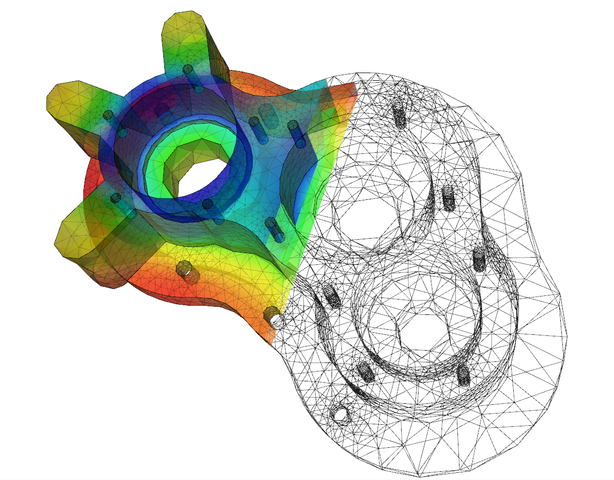
\includegraphics[scale=0.2]{imagenes/614px-Elmer-pump-heatequation.png} 
\caption{Ejemplo de uso de Elmer. \cite{ElmerpumpheatequationPng}}
 \label{fig:Elmer-pump-heatequation.png}
\end{figure}

\begin{figure} %con el [H] le obligamos a situar aquí la figura
\centering
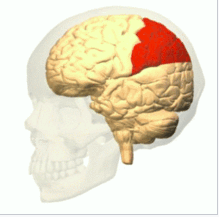
\includegraphics[scale=0.6]{imagenes/lobulo_parietal.png} 
\caption{Modelo 3D del Lobulo parietal, fuente Wikipedia} \label{fig:lobulo_parietal.png}
\end{figure}

\subsection{ Representaciones de Objectos}
Las dos representaciones tiene sus ventajas y desventajas. La representación de fronteras 
es una representación menos real y con más limitaciones en cuanto al cálculo de propiedades y estados del objeto pero permite una apariencia tan detallada como quieras con un menor coste de memoria del ordenador así como de tiempo de computo para la generación del objeto. Pero por otro lado tenemos la representación volumétrica que sí nos permite representar el objeto en su totalidad, es decir, incluyendo las capas que deseemos así como todas las propiedades de las distintas partes del interior del objeto. De esta forma es posible asignar distintos colores y transparencias a una cabeza humana para visualizar las partes que deseemos y tener una representación más fiel. Nuestro trabajo utiliza modelos de frontera, en concreto, mallas poligonales.\\

Otro apartado a tener en cuenta es forma de dibujar la malla. Pero primero es definir que es una malla, una malla poligonal. Una malla poligonal es un conjunto de vértices, aristas y caras, donde los vértices están unidos a través de aristas formando caras que a su vez forman una figura poligonal (ver ejemplo \ref{fig:mesh_overview.png}). Una de las características principales de una malla es la forma en la que se forman las caras dependiendo del número de aristas necesarias para formarlas. La forma más básica es el triángulo, que requiere la unión de tres vértices con tres aristas. La siguiente sería los \textit{quads} que requiere la unión de cuatro vértices con cuatro aristas. Y por último poligonal, que se compone de cinco o más vértices y el mismo número de aristas para formar una superficie. Cada forma tiene sus propiedades y requisitos, por ello la más utilizada sin entrar en muchos detalles es la forma más básica el triángulo ya que siempre está contenido en un plano. De hecho, el triángulo es el símplice 2D. Además permite una representación muy sencilla y rápida.\\

\begin{figure} %con el [H] le obligamos a situar aquí la figura
\centering
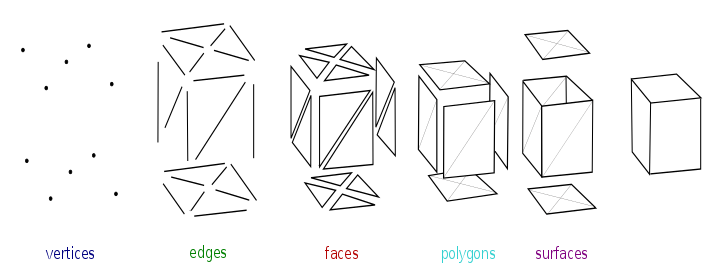
\includegraphics[scale=0.4]{imagenes/Mesh_overview.png} 
\caption{Partes de una malla poligonal, fuente Wikipedia (\cite{lobsterbakeEnglishLicensingCcbysa32009})} \label{fig:mesh_overview.png}
\end{figure}

Desde la definición de las mallas de triángulos se han investigado la forma de optimizar los recursos y acelerar los cálculo que se realizan sobre la misma. Algunas mejoras se centran en la forma de definir las aristas para la exploración y recorrido de la malla. Las mallas actuales con cierto grado de realismo cuentan fácilmente con varios miles de caras, que significa que requiere al menos tres veces más de vértices y de aristas, por esto es muy importante optimizar la forma en que se almacenan los datos y la forma de moverse por la malla. Una aproximación de movimiento por barrido, es decir, partiendo del primer vértice y luego al siguiente vértice para para ver si están conectados es una búsqueda exponencial del tipo $O(n^n)$ una búsqueda muy costosa.

La resolución de este problema derivó en la aparición de nuevas estructuras de datos para las aristas. Uno de los resultados fue las \textit{aristas aladas} una representación que guarda la información de donde procede la arista y a donde va, es decir, los dos vértices que delimitan la arista y de las aristas siguiente y anterior. Esta estructura optimiza la navegación por la malla pero tiene el inconveniente de que almacena dos veces cada arista, la que va del vértice $i$ al vértice $i+1$ y la que va del vértice $i+1$ al vértice $i$. De esté modo no es muy eficiente el almacenamiento de la estructura (ver figura \ref{fig:winger_edge.png}).\\ 


\begin{figure} %con el [H] le obligamos a situar aquí la figura
	\centering
	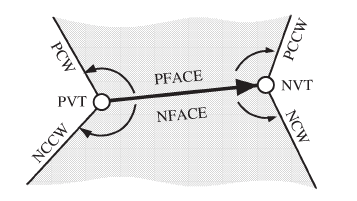
\includegraphics[scale=0.4]{imagenes/winger_edge.png} 
	\caption{Esquema de una arista alada, fuente (\cite{kettnerUsingGenericProgramming1999})} \label{fig:winger_edge.png}
\end{figure}


La siguiente solución que se dio a este problema fueron las \textit{''semi-aristas aladas``} definidas en (\cite{kettnerUsingGenericProgramming1999} y \cite{campagnaDirectedEdgesScalable1998} ) solucionan el problema del doble almacenamiento y además permiten un mayor conocimiento de la vecindad de la arista. Esta estructura supone que una arista está compuesta de dos semi-aristas una en cada dirección. Además se adjunta a cada semi-arista la información de la semi-arista siguiente, la anterior y la opuesta, entendiendo la opuesta como la semi-arista complementaria de la arista (ver figura \ref{fig:halfedge_small.png}). 

\begin{figure} %con el [H] le obligamos a situar aquí la figura
	\centering
	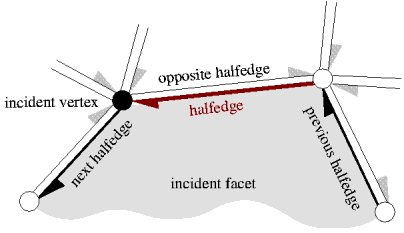
\includegraphics[scale=0.4]{imagenes/halfedge_small.png} 
	\caption{Esquema de una semi-arista alada, fuente The Computational Geometry Algorithms Library (\cite{CGAL12Halfedge})} \label{fig:halfedge_small.png}
\end{figure}

\subsection{APIs en informática gráfica}
En los años noventa la compañía \textit{``Silicon Graphics, Inc''} (SGI) desarrollaron la primera API para gráficos libre, OpenGL, del inglés Open Graphics Library \cite{OpenGLOverview}. SGI liberó una API potente para la época que facilitaba mucho la tarea del programador a la hora de programar todo el entorno de los gráficos. Rápidamente se estableció como la API de informática gráfica más usada, estableció algunos conceptos y formas de trabajar que se utilizan a día de hoy y que siguen inmutables y gran parte del software de gráficos utiliza directamente OpenGL o se basa en el. Un elemento fue la arquitectura de debían seguir para programar gráficos, además de establecer el cómo y que uso tiene del cauce gráfico. OpenGL ha ido sacando actualizaciones y mejoras sobre si mismo hasta llegar a la versión 4.5, pero su pensamiento base e ideas principales se mantienen.\\

En el año 2000 nació \textit{``Khronos Group''} (\cite{KhronosGroup2018}) una compañía para la cooperación y desarrollo del entorno virtual de la informática gráfica bajo los estándares abiertos. Se hicieron cargo de OpenGL y a partir de el desarrollaron más APIs para el desarrollo de gráficos, como fueron: \texttt{WebGL, OpenCL, SPIR, OpenVR, etc}. Entre ellas la más actual ha sido \texttt{Vulkan} una API que liberaron en febrero de 2016 para adaptar OpenGL al hardware moderno y actualizar su núcleo con las nuevas tecnologías. Las principales ventajas de \texttt{Vulkan} sobre \texttt{OpenGL} es que está pensado para aprovechar al máximo el hardware actual, en los años noventa casi todos o los más habituales eran los procesadores con un solo núcleo  y cauces muy lentos entre la tarjeta gráfica (GPU) apenas con memoria (\cite{NVIDIANV1}) y el procesador(CPU), por ello se destinaba casi todo el computo a la GPU y un poco de control en la CPU. \texttt{Vulkan} se sustenta en los procesadores de varios núcleos y cauces muy rápidos además de GPUs con arquitecturas superiores en cuanto paralelización y mucho mayor espacio de memoria. De esta forma \texttt{Vulkan} permite una paralelización muy superior a \texttt{OpenGL} entre otras ventajas.\\

\subsection{Objetivo del proyecto}
Este proyecto consta principalmente del procesado geométrico de una malla de triángulos. El procesado geométrico sobre una malla ofrece una gran versatilidad de operaciones sobre la malla tales como (Curso sobre procesado geométrico de la Universidad de Stanford \cite{mirelaben-chenCS468GeometryProcessing}):
simplificación de una malla, mejora de la calidad de una malla, deformaciones, mapeado de texturas, reconstrucciones de partes de la malla, detección de propiedades, etc. El campo del procesado geométrico es realmente amplio y con una infinidad de aplicaciones posibles.En este proyecto nos centramos en las operaciones más básicas pero muy importantes, como son la simplificación de una malla, voltear aristas cambiando así la topología de la malla (entre otras).

\subsubsection{Desarrollo de un Motor Gráfico}
Un apartado importante es el desarrollo de un motor gráfico que nos permita soportar mallas de triángulos. Este motor tiene que estar centrado en el procesado geométrico de las mallas y por tanto tiene que contener una una estructura de datos capaz de soportar dicha tarea. El procesado geométrico de mallas requiere de algoritmos de simplificación, modificación y operaciones de cálculo sobre la malla, estos algoritmos suelen ser bastante costosos en cuanto a recorrer la malla y aplicar operaciones por tanto la optimización de la estructura de datos y métodos aplicados debe ser muy eficiente. Para la estructura de datos se utilizará la estructura de semi-aristas aladas que proveen de una navegación por la malla eficaz y eficiente permitiendo así modificaciones más fáciles y de mejor eficiencia que otras estructuras \cite{kettnerUsingGenericProgramming1999}, obteniendo un buen resultado para el procesado geométrico.

\subsubsection{Visualizador de Mallas}
Otro aspecto del proyecto es la parte del visualizador de mallas o renderizador, cuya labor es generar la malla de triángulos en pantalla para que el usuario pueda verla. El visualizador se realizará utilizando las librerías de OpenGL y las tecnologías de QT que encapsulan el funcionamiento laborioso de OpenGL. El visualizador tiene que contar con operaciones básicas para el usuario como son el movimiento de la cámara por el espacio para poder visualizar como se deseé la malla y desde el angulo que prefiera.

\subsubsection{Procesamiento Geométrico}
Estudio e implementación de operaciones de procesamiento geométrico, en concreto de operaciones de simplificación de aristas y caras. Estas operaciones están enfocadas a mejorar la eficiencia de la malla mediante la reducción del número de aristas y de caras pero manteniendo siempre las propiedades de la malla, así como su forma en medida de lo posible.

Los algoritmos de simplificación son muy utilizados en las areas de ``Levels of details'' y optimización de escenas. Donde se debe de mantener un framerate, tasa de imagenes por segundo, sin que el usuario note el procesado. Estos algoritmos permiten la generación de escenas de películas y videojuegos cada vez más realistas manteniendo un consumo de recursos Hardware considerable.

\subsubsection{Decimation}
Todos los objetivos anteriores cada uno importante por si mismo deben juntarse para producir una API capaz de procesar el algoritmo de procesado geométrico \texttt{Decimation}, que dado un parámetro de tasa de reducción de triángulos especificado por le usuario aplique un algoritmo de simplificación de aristas y caras y lo muestre por la pantalla, a través de un visualizador de mallas. Por decirlo de algún modo es juntar todos los objetivos anteriormente descritos y construir un flujo de trabajo conjunto para un objetivo concreto. Aquí se probará la eficiencia y las operaciones implementadas en la estructura de datos.
%
\chapter{ Especificación de requisitos}

\section{Objetivos}

\begin{enumerate}[label=\textbf{\textit{OBJ-\arabic*}}]
	\item El sistema a desarrollar es un motor gráfico capaz de renderizar y mostrar elementos geométricos al usuario a partir de un fichero con formáto ply que contenga una malla de triángulos.
	\item El motor gráfico debe permitir la interacción con el usuario de una forma cómoda y agradable mediante la interfaz de usuario que muestre la malla en su estado actual y una cámara para poder visualizarla desde el ángulo deseado.
	\item Estudio e implementación de algoritmos de procesado geométrico para la simplificación de una malla mediante la reducción de aristas y caras. 
	\item Implementación de la estructura de datos de semi-aristas aladas con las operaciones necesarias para una correcta navegación e interacción con la malla de triángulos.
	\item Implementación y análisis del algoritmo de procesado geométrico ``Decimation'' con varias mallas de triángulos. Donde el usuario pueda especificar una tasa de reducción que se vaya a aplicar a la malla.
	
\end{enumerate}

\newpage
\section{ Requisitos Funcionales}


\begin{enumerate}[label=\textbf{\textit{RF-\arabic*}},ref=RF-\arabic*]
	\item \label{RF1}Almacenar mallas de triángulos.
	
	\begin{enumerate}[label*=\textbf{\textit{.\arabic*}}]
		\item \textit{Almacenar los vértices de la malla.} El modelador tiene una estructura de datos para la manipulación de los vértices \ref{RI1}, \ref{RI2}. 
		\item \textit{Almacenar las caras que componen la malla.} El modelador almacena las caras de la malla en una estructura de datos adecuada \ref{RI3}.
		\item \textit{Almacenar las aristas de la malla.} El modelador posee una estructura de datos basada en semi-aristas aladas para las aristas \ref{RI2}. 
	\end{enumerate}
	
	\item Lectura de mallas de triángulos \ref{RI3}.
		\begin{enumerate}[label*=\textbf{\textit{.\arabic*}}]
		\item \textit{Leer ficheros en formato ``Polygon File Format''.} El modelador tiene que poder leer de un fichero externo con el formato ``Polygon File Format'', sin perder la información contenida en el fichero.
		\end{enumerate}
	
	\item Interacción con la escena 3D \ref{RI3}.
	\begin{enumerate}[label*=\textbf{\textit{.\arabic*}}]
		\item \textit{Poder tener interacción con la escena 3D.} La API genera una escena donde se muestran mallas 3D y el usuario tiene que poder navegar por la escena.
	\end{enumerate}

	
	\item Mostrar información al usuario de mallas de triángulos.
	\begin{enumerate}[label*=\textbf{\textit{.\arabic*}}]
		\item \textit{Número de triangulos.} Mostrar al usuario el número de vértices que contiene la malla actual.  
		\item \textit{Número de aristas.} Mostrar al usuario el número de aristas que contiene la malla actual.
		\item \textit{Número de caras.} Mostrar al usuario el número de caras que contine la malla actual.
		
	\end{enumerate}
			
	
	\item Realizar operaciones de procesado geométrico sobre la malla.
		\begin{enumerate}[label*=\textbf{\textit{.\arabic*}}]
		\item \textit{Converger un vértice en otro.} El modelador tiene que permitir converger un vértice al vértice que apunta su semi-arista alada.
		\item \textit{Optimización de una malla.} Mediante un parámetro de reducción optimizar la malla para que alcance una reducción del número de triángulos que la componen al deseado.
		\end{enumerate}	
	
\end{enumerate}


\section{ Requisitos No Funcionales}


\begin{enumerate}[label=\textbf{\textit{RNF-\arabic*}},ref=RNF-\arabic*]
	\item Que el renderizado sea rápido.
	\item Modularizar el código para su posible reutilización.
	\item Que la interfaz sea agradable.
	\item Tiene que ser intuitivo para el usuario.
	\item La visualización de los datos ha de hacerse en tiempo real.
	\item El código ha de ser abierto.
	\item El código tiene que estar bien documentado.
	
	
	
\end{enumerate}

\section{ Requisitos de Información}


\begin{enumerate}[label=\textbf{\textit{RI-\arabic*}},ref=RI-\arabic*]
	\item \label{RI1} Vértices: Listado de vértices. Un vértice es una posición $XYZ$ y una referencia a la semi arista alada que incide en el vértice.  
	\item \label{RI2} Semi-Arista alada: 
	\item \label{RI3} Caras: Listado de 3-tuplas que hace referencia a los vércites que delimitan cada una de las caras.
	\item \label{RI4} Normales de cara: vector unitario que define a dirección de la cara \cite{llcFaceVertexNormal}.
	\item \label{RI5} Color de vértice: define el color en escala RGB de un vértice.
	%\item \label{RI4} 
	
	
	
\end{enumerate}
%
\chapter{Planificación}

\section{ Planificación inicial}
Se ha realizado una planificación inicial con la fecha objetivo del 14 de Junio del 2018. Se utiliza la herramienta de ``Gantt Project'' para la planificación y se obtiene el diagrama de planificación inicial, ver figura \ref{fig:planificacion_inicial.png}. La planificación está agrupada en varios módulos:\\

\begin{enumerate}
	\item Aprendizaje de la tecnología \textit{Vulkan}. Se destinará una gran cantidad de tiempo para aprender sobre esta nueva tecnología de informática gráfica. Es una tecnología que se liberó el año 2016 (\cite{KhronosReleasesVulkan2016}), es por ello que he destinado gran parte del tiempo a su aprendizaje a un nivel básico.
	
	\item Entorno de trabajo, al ser \textit{Vulkan} una nueva tecnología la instalación de las librerías y configuración de las mismas, está aun muy verde y hay poca información. En tiempo asignado para la correcta configuración y puesta en funcionamiento es de 7 días.
	
	\item Desarrollo de un renderizador. Este modulo cuenta con el desarrollo de una api para mostrar objetos 3D a partir de una malla de triángulos en pantalla. Hay que gestionar la escena, la posición de la cámara y las luces, además de toda la configuración requerida por la API gráfica \textit{Vulkan}. 
	
	\item Modelado de Mallas. La parte de modelación permite seleccionar un vértice del objeto y poder moverlo libremente.
	\item Procesado Geométrico, es la parte principal del trabajo y por tanto para poder aplicar algunos algoritmos se le asigna más tiempo que a ninguna otra tarea.
	
	\item Desarrollo de la memoria. Se va a realizar en paralelo durante todo el proceso de desarrollo de la API.
\end{enumerate}

\begin{figure} %con el [H] le obligamos a situar aquí la figura
	\centering
	\hspace*{-1.6in}
	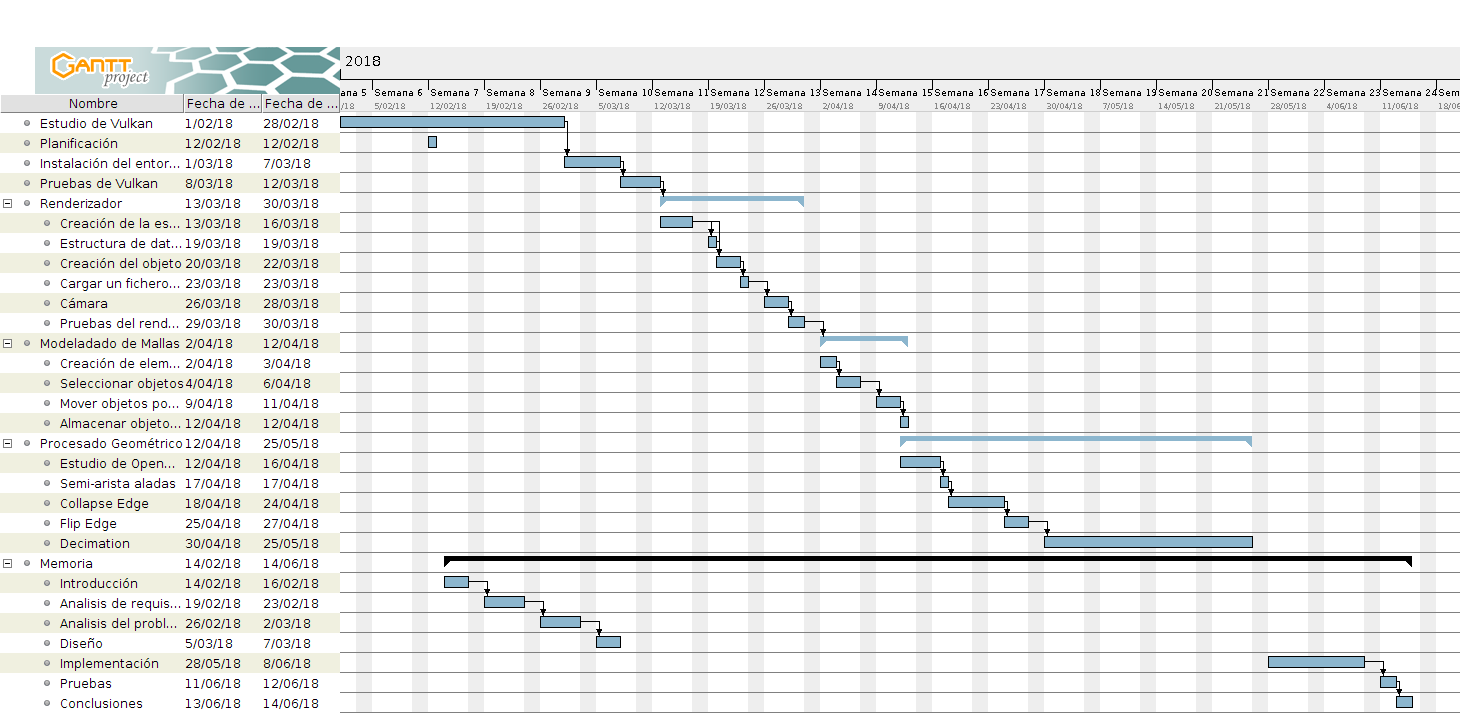
\includegraphics[scale=0.38]{imagenes/Modelator_GP_planning.png} 
	\caption{Diagrama de planificación inicial, por el software ``Gantt Project''} \label{fig:planificacion_inicial.png}
\end{figure}

\subsection{ Avance del proceso}
El trabajo se inició como esta previsto, el primer día de Febrero de 2018, con la documentación y tutoriales de ``Khronos Group'', en \cite{VulkanSubgroupTutorial2018}, \cite{IntroductionVulkanTutorial}, \cite{LunarXchange} la cual es el tutorial oficial que proveé \textit{Khronos Group} para comprobar que funciona correctamente la instalación. Durante el mes de Febrero estuve estudiando el funcionamiento de los buffers, declaraciones y otros elementos a tener en cuenta. Se realizó el trabajo asignado sin problemas durante este periodo.\\

A partir de Marzo empecé con la instalación del entorno en un Sistema Operativo Windows 10 y en otro basado en Linux (Ubuntu 16.04LST, en concreto). Esta parte se componía de la instalación de los IDEs: \texttt{QTCreator 4.5}, Drivers de \texttt{Vulkan} distribuidos por \texttt{``Lunar Xchange''} y instalación de la librería \texttt{OpenMesh}. Además de la correcta visibilidad por parte de las librerías requeridas hacia el compilador. La instalación en ambos sistemas operativos de \texttt{QTCreator} y el driver de \texttt{Vulkan} se hicieron con forme estaba previsto, pero la configuración de las variables de entorno para la correcta compilación del \texttt{Vulkan} no se completó, lo que derivó en un retraso cada vez más grande. Esta parte estaba prevista completarla en una semana por los problemas que suelen dar las instalaciones de elementos relativamente nuevos, pero aun así no se pudo realizar y a principios de Abril se puso el retraso en conocimiento del Tutor para conseguir arreglarlo. Todo el trabajo ya tenía un retraso de un mes, y en Abril tampoco se consiguió que funcionara correctamente por lo que a finales de Abril se decidió cambiar el driver gráfico a OpenGL y volver a re-calcular el proyecto. Por lo que la planificación inicial no se pudo seguir.


\section{ Planificación inicial con OpenGL}
Dado el cambio del driver gráfico de \textit{Vulkan} por \textit{OpenGL} se ha realizado una nueva planificación y re-estructuración de las tareas pero manteniendo el objetivo principal del proyecto quedando como se muestra en la figura \ref{fig:planificacion_final.png} y \ref{fig:planificacion_final2.png}.\\

Ahora en vez de utilizar la tecnología de \textit{Vulkan} usaremos la última versión de \textit{OpenGL 4.5} aprendiendo a controlar y utilizar los \textit{buffers} y demás características propias de esta versión.

\begin{figure} %con el [H] le obligamos a situar aquí la figura
	\centering
	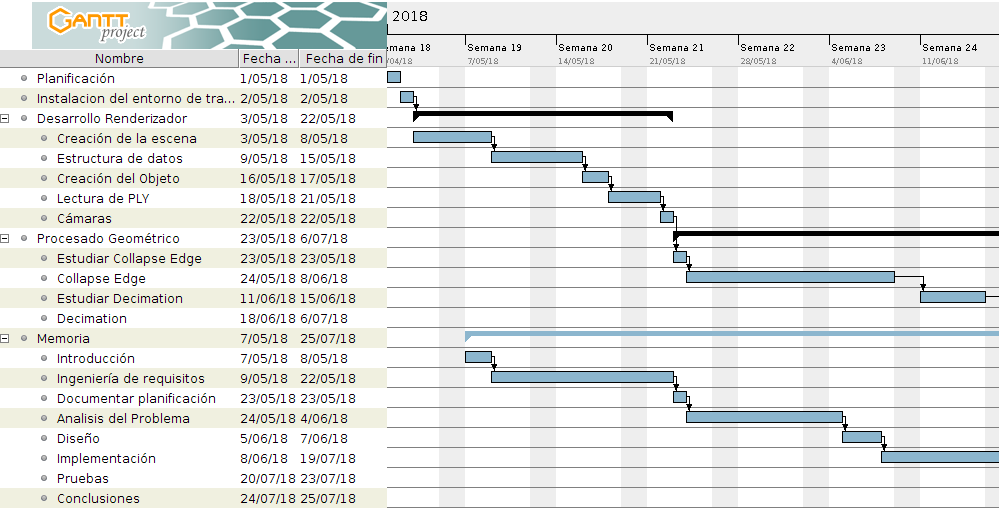
\includegraphics[scale=0.4]{imagenes/Modelator_GP_planning_modi.png} 
	\caption{ (1/2) Diagrama de planificación final, por el software ``Gantt Project''} \label{fig:planificacion_final.png}
\end{figure}

\begin{figure} %con el [H] le obligamos a situar aquí la figura
	\centering
	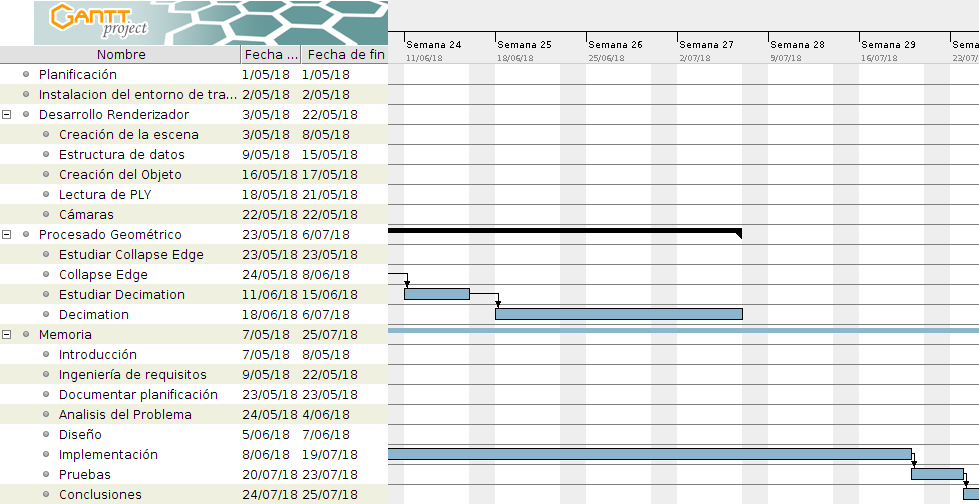
\includegraphics[scale=0.4]{imagenes/Modelator_GP_planning_modi2.png} 
	\caption{ (2/2) Diagrama de planificación final, por el software ``Gantt Project''} \label{fig:planificacion_final2.png}
\end{figure}

\subsection{ Detalle de los procesos}

Los primeros días de mayo se realizó una nueva planificación teniendo en cuenta los nuevos plazos de tiempo y el cambio de driver gráfico resultando de la siguiente forma el progreso.\\

\begin{itemize}
	\item[] \textbf{Planificación (1 de Mayo)}: Se planificó todo el trabajo tareas a realizar sin ningún problema.
	
	\item[] \textbf{Instalación del entorno de trabajo (2 de Mayo)}: Al ser un entorno del que se tiene una base, se realiza en el tiempo establecido.
	
	\item[] \textbf{Desarrollo del Renderizador}: está compuesto por las sub-tareas:
	\begin{enumerate}
		\item \textbf{Creación de la escena (del 3 de Mayo al 8 de Mayo)}: se requiere crear una escena 3D donde poder visualizar y crear los objetos.
		
		\item \textbf{Estructura de datos (del 9 de Mayo al 15 de Mayo)}: Creación de toda la estructura de clases y atributos necesaria para la API, y sus pruebas oportunas.
		
		\item \textbf{Creación del Objeto (del 16 de Mayo al 17 de Mayo)}: Crear un objeto básico y su visualización.
		
		\item \textbf{Lectura de PLY (del 18 de Mayo al 21 de Mayo)}: Poder leer un objeto 3D desde un fichero en formato ``ply'' y almacenarlo en la estructura de datos propia.
		
		\item \textbf{Cámaras (el 22 de Mayo)}: implementación de las cámaras de la escena y su movimiento.
		
	\end{enumerate}
	
	\item[] \textbf{Procesado Geométrico}: estudio e implementación de algoritmos para el procesado geométrico de la malla:
	\begin{enumerate}
		
		\item \textbf{Estudiar Collapse Edge (el 22 de Mayo)}: comprender cómo funciona la operación de colapsar un vértice en otro a través de una semi-arista.
		
		\item \textbf{Collapse Edge (del 24 de Mayo al 8 de Junio)}: implementación del algoritmo de collapse edge y probar que funciona correctamente.
		
		\item \textbf{Estudiar ``Decimation'' (del 11 de Junio al 15 de Junio)}: comprender el funcionamiento del algoritmo para optimizar la malla a través de la eliminación de vértices y aristas del objeto.
		
		\item \textbf{``Decimation'' (del 18 de Junio al 6 de Julio)}: implementación del algoritmo de ``decimation'' y todos los módulos que requiera. Así como su testeo.
	\end{enumerate}

	\item[] \textbf{Memoria}: desarrollo de la memoria del proyecto:
	\begin{enumerate}
		\item \textbf{Introducción (del 7 de Mayo al 8 de Mayo)}: introducción de la memoria y la motivación que tengo para realizar este proyecto.
		
		\item \textbf{Ingeniería de Requisitos (del 9 de Mayo al 22 de Mayo)}: todo el proceso de Ingeniería de Software con respecto al diseño previo que requiere un sistema software así como las necesidades de la aplicación.
		
		\item \textbf{Documentar planificación (el 23 de Mayo)}: documentar cómo se ha realizado la planificación y cuales van a ser las tareas a desarrollar en cada fase y durante cuanto tiempo.
		
		\item \textbf{Análisis del Problema (del 24 de Mayo al 4 de Junio)}: analizar detalladamente el problema que se ha detectado y como se va a solucionar.
		
		\item \textbf{Diseño (del 5 de Junio al 7 de Junio)}: realizar todo el diseño software necesario para la implementación del software.
		
		\item \textbf{Implementación (del 8 de Junio al 19 de Julio)}: detallar el proceso de implementación y cómo están realmente implementado el software.
		
		\item \textbf{Pruebas (del 20 de Julio al 23 de Julio)}: documentar cómo se han realizado las pruebas oportunas y en que consisten.
		
		\item \textbf{Conclusiones (del 25 de Julio al 26 de Julio)}: describir mis propias conclusiones al realizar y terminar el proyecto.
	\end{enumerate}
	
\end{itemize}

\subsection{ Avance del proceso}

\textbf{Instalación del entorno de trabajo:} se ha realizado en el plazo previsto, al ser un entorno ya conocido no aparecen ninguna incidencia.\\

\textbf{Desarrollo del Renderizador:} las primeras tareas se realizaron en tiempo y se consiguió el renderizado de un objeto 3D en menos tiempo del planificado, pero al final de proceso se detecta que no se está utilizando correctamente la API gráfica de OpenGL 4.5 y se procede a cambiarla, lo que provoca que se finalice la tarea el 31 de Mayo.\\

\textbf{Procesado Geométrico:} Se inició el 4 de Junio por el retraso ocasionado por la etapa anterior. En detalle el estudio del \textit{``collapse edge''} se llevo a cabo sin problemas y en el tiempo previsto. Pero la implementación tuvo un problema de diseño base en la implementación de la estructura de datos, y se tuvo que retocar la estructura de datos lo que retraso el trabajo dos días. La estructura no estaba originalmente bien construida para soportar las referencias entre los distintos objetos. El resto de la implementación se llevo a cabo en un día más de lo previsto, por lo que se retrasó el trabajo total de esta parte en casi una semana.\\

La segunda parte del procesado geométrico consistía en el entendimiento y desarrollo de un algoritmo de optimización, ``decimation''. El estudio fue complejo ya que mucha documentación son artículos de revistas científicas con un nivel de abstracción bastante alto. El estudio estaba previsto en 4 días pero al final fueron 6 días. 
Una vez entendido el algoritmo se procedió a su implementación en la estructura desarrollada anteriormente.\\

La implementación del algoritmo se realizó con cautela y probando cada método con una malla pequeña y conocida. Aun así se requirieron dos semanas para su desarrollo, puesto que además había que calcular valores auxiliares como el error generado por eliminar una arista de la malla. Una vez terminado se probó con una malla pequeña y conocida con poca reducción y funcionó, pero cuando se realizo la prueba a una malla de verdad con miles de caras y elementos surgió un problema de memoria dinámica. Este problema ocasiono un retraso de más de una semana hasta que se descubrió cual era el origen y a partir de ahí se procedió a evaluar la mejor forma de solucionarlo. Se decidió optar por cambiar las estructuras base de vectores por listas doblemente enlazadas, por lo que habría que cambiar partes de la estructura de datos. En total se retrasó la tarea dos semanas más de trabajo real. Pero como se pausó el arreglo del fallo para continuar con el desarrollo de la memoria en agosto, se terminó la tarea el 4 de septiembre. \\

\textbf{Desarrollo de la Memoria:}
La memoria se empezó a desarrollar al principio de mayo, el capítulo de introducción e Ingeniería de Requisitos se terminó en el plazo previsto y se mandó a revisión por el tutor. El tutor respondió con los cambios que consideró necesarios y se procedió de inmediato a revisarlos e integrar los que se vieron necesarios. Terminando estos capítulos a finales de mayo.

La documentación de la planificación se realizó en primera instancia planificando los tiempos y las tareas, pero con los problemas surgidos se ha ido completando esta sección con forme se terminaban las tareas implicadas.

El análisis como ya se había realizado fue perfectamente en el tiempo dado, se plasmo las ideas obtenidas durante esta tarea y se realizó una documentación precisa.

El apartado de diseño se quedó más sencillo ya que al ser una API gráfica y contar con un flujo de trabajo con pocas operaciones de procesado pero complejas se optó por realizar el diagrama de clases para mostrar la estructura del sistema y la organización de la arquitectura.

La implementación una vez realizada se documentó sobre como quedaron las clases y objetos y porqué se construyen de esa forma. Esta partes se desarrollo en el tiempo indicado.

Las pruebas y conclusiones dado que se retrasó todo el trabajo de implementación se tuvo que retrasar esta parte también hasta tenerlo todo funcionando al 100\%. Se realizó en menos tiempo del establecido, ocupando solo dos días y terminando así el proyecto antes de la entrega.


%
\chapter{ Análisis}

\section{ Análisis del Problema}
El principal problema que se plantea solventar es el desarrollo de una API gráfica que sea capaz de ilustrar el funcionamiento de algoritmos de simplificación geométrica. Este desarrollo implica el estudio de las últimas tecnologías y metodologías de programación gráfica, programación orientada a objetos así como de estructuras de datos.\\

Una API es una interfaz de programación de aplicaciones, o su nombre en ingles del que proceden las siglas: \textit{Application Programming Interface}. La API no es más que un software que encapsula una serie de funciones para volver a usarse más adelante favoreciendo la reusabilidad del software y siguiendo los principios de la Ingeniería de Software (\cite{sommervilleSoftwareEngineeringGlobal2016}) además de una documentación sobre como utilizar correctamente dicho software.\\ 


Para solucionar el problema principal se ha dividido el proyecto en dos etapas, la primera consiste en crear un software que muestre al usuario imágenes de objetos 3D generadas a partir de un fichero que define una malla de triángulos según las especificaciones de ``Polygon File Format'', también llamado \textit{render} y la segunda el estudio, implementación y aplicación de algunos algoritmos de simplificación geométrica a mallas que previamente han sido importadas en el render.

\subsection{ Renderizador}
El primer sub-problema al que me enfrento es la de crear un renderizador capaz de mostrar mallas de triángulos en tres dimensiones y que permitan al usuario una visualización cómoda y fácil. Para ello necesito una API gráfica para la generación y manejo de los gráficos y un framework de desarrollo. Un claro ejemplo de render es \texttt{Meshlab} (ver ejenplo \ref{fig:meshlab_presentacion.png}). \texttt{Meshlab} es un software muy avanzado de gráficos pero yo solo me centraré en  cumplir con los requisitos especificados en el capitulo segundo.\\

\begin{figure} %con el [H] le obligamos a situar aquí la figura
	\centering
	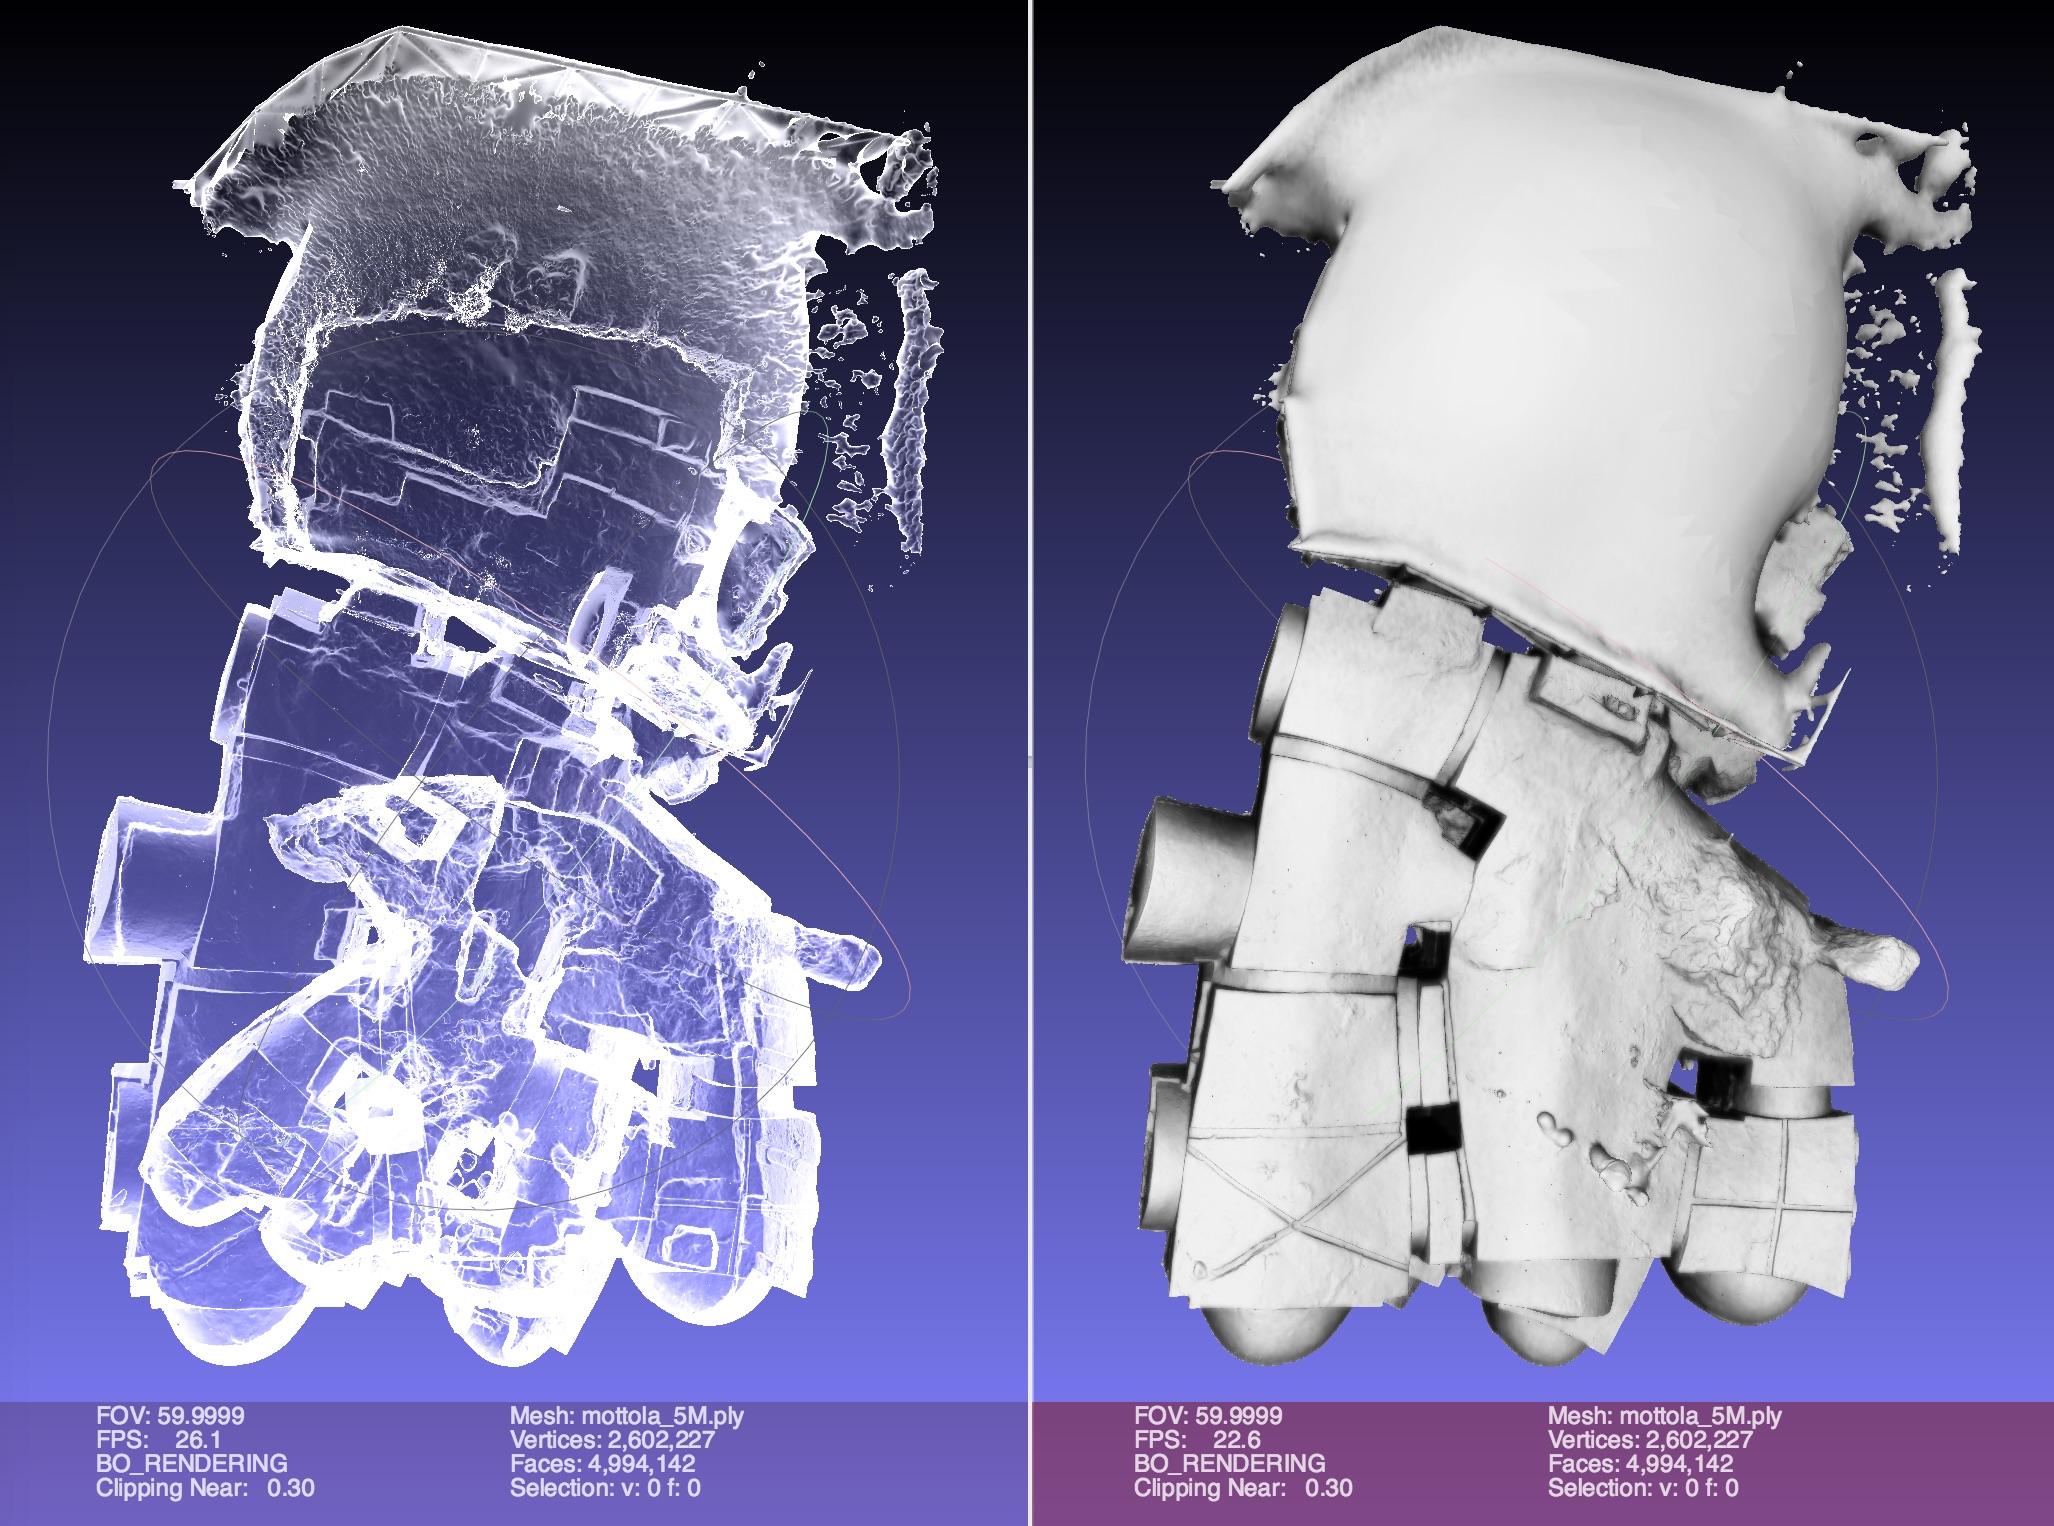
\includegraphics[scale=0.15]{imagenes/Presentation.jpg} 
	\caption{ Imagen renderizada por MeshLab \cite{cignoniMeshLabOpenSourceMesh2008}} \label{fig:meshlab_presentacion.png}
\end{figure}

Para cumplir el primer requisito funcional (\ref{RF1}) se debe de realizar una muy buena gestión de la estructura de datos que almacenará todos los elementos y atributos de la malla de triángulos. Si analizamos con más detalle la malla vemos que está compuesta principalmenete de la geometría y la topología. Como indica Martti Mäntylä \cite{marttimantylaIntroductionSolidModeling}: \textquotedblleft La geometría de un modelo viene dada por las coordenadas de aquellos puntos que están sobre la superficie y la topología de un modelo es cómo se organiza la geometría para dar lugar a una superficie \textquotedblright. De modo que sintetizamos la geometría en los vértices y la topología en las aristas que unen dichos vértices formando la malla triangular. Por tanto para almacenar los vértices usaremos la siguiente estructura:\\

Vértice:

\begin{algorithmic}
\hrule
	\State $Atributos$
	\State \hspace{1cm} $position : 3-Tupla(Real)$
	\State \hspace{1cm} $color : 3-Tupla(Real)$
	\State \hspace{1cm} $halfEdgeIn : HalfEdge[]$
	\State \hspace{1cm} $halfEdgeOut : HalfEdge[]$
	\State \hspace{1cm} $id : Natural$
\hrule
\end{algorithmic}
\vspace*{1cm}

Definiendo en más detalle los atributos:
\begin{itemize}
	\item \textbf{position}: representa las coordenadas X,Y,Z de un vértice en el espacio.
	\item \textbf{color}: indica en en formato RGB de cada vértice.
	\item \textbf{halfEdgeIn}: array de referencias a las semi-aristas aladas que inciden en el vértice.
	\item \textbf{halfEdgeOut}: array de referencias a las semi-aristas aladas que salen del vértice.
	\item \textbf{id}: Entero que identifica al vértice.
\end{itemize}

Para en caso de las aristas, como ya se introdujo en el capitulo 1 pero lo detallaremos más, se ha tomado la decisión de utilizar una estructura más moderna que las aristas normales y son las semi-aristas aladas. Esta decisión está apoyada por las sustanciales mejoras que aporta esta estructura frente a otras. En comparación con la de aristas dirigidas como se dice en el estudio de ``Using generic programming for designing a data structure for polyhedral surfaces'' (\cite{kettnerUsingGenericProgramming1999}) y en ``Directed Edges—A Scalable Representation for Triangle Meshes'' (\cite{campagnaDirectedEdgesScalable1998}) donde se exponen las ventajas, algunas como la facilidad de navegación por la malla. Este aspecto es clave a la hora de aplicar algoritmos de procesado geométrico donde la navegación por la malla es una operación muy utilizada y si una estructura de datos facilita dicha operación en tiempo, facilidad y potencia es una elección muy importante. Es cierto que las aristas aladas son muy parecidas a las semi-aristas aladas a primera vista, pero si se examinan con más detalle se puede observar un problema que ocurre en las aristas aladas. La topología que une dos vértices se orienta en el caso de las aristas dirigidas cómo, una arista que va del vértice $a$ al vértice $b$ con toda la información correspondiente. Además tiene que existir otra arista que vaya del vértice $b$ al vértice $a$ con prácticamente los mismos datos. Lo que ocasiona una repetición de información cuando lo analizamos a nivel global de toda la malla, pues por cada arista se están repitiendo el puntero a las caras adyacentes y las referencias a las aristas anteriores y siguientes, pero en orden contrario. Esta duplicación de información desaparece con las semi-aristas aladas pues al dividir cada arista dirigida en dos una en el mismo sentido y otra con el sentido contrario ya solo se almacena la información justa. Además otra ventaja es que no hace falta comprobar la orientación de la arista puesto que al estar ya dividida en dos, una para cada sentido ya está implícito en cada semi-arista. \\

Ahora es necesario implementar la estructura de semi-aristas aladas y se ha diseñado de la siguiente forma:\\

Semi-Aristas Aladas:
\begin{algorithmic}
	\hrule
	\State $Atributos$
	\State \hspace{1cm} $id : Integer$
	\State \hspace{1cm} $vertexIn : Vertice$
	\State \hspace{1cm} $vertexOut : Vertice$
	\State \hspace{1cm} $face : Cara$
	\State \hspace{1cm} $nextHalfEdge : HalfEdge$
	\State \hspace{1cm} $opositeHalfEdge : HalfEdge$
	\State \hspace{1cm} $previousHalfEdge : HalfEdge$
	\hrule
\end{algorithmic}
\vspace*{1cm}

Los atributos definen lo siguiente:
\begin{itemize}
	\item \textbf{id}: Entero que identifica a la semi-arista alada.
	\item \textbf{vertexIn}: referencia al vértice sobre el que incide la semi-arista.
	\item \textbf{vertexOut}: referencia al vértice del que sale la semi-arista alada.
	\item \textbf{face}: referencia a la cara sobre la que incide.
	\item \textbf{nextHalfEdge}: referencia a la semi-arista siguiente, entendiendo siguiente como la semi-arista que sale del vértice sobre el que incide e incide sobre la misma cara.
	\item \textbf{opositeHalfEdge}: referencia a la semi-arista contraria, es decir, que tiene la misma posición pero la dirección opuesta.
	\item \textbf{previousHalfEdge}: referencia a la semi-arista anterior.
\end{itemize}

Una vez tenemos los vértices y las semi-aristas definidas cómo se van a implementar, el siguiente elemento que surge son las caras. Una cara es una superficie delimitada por tres semi-aristas seguidas que unen tres vértices. Las caras en nuestro caso solo se necesitan para el procesado de mallas, ya que para la renderización nos basta con los vértices y las semi-aristas. Pero para el procesado sí que es necesario guardar cierta información para la navegación de la malla.\\
\newpage
Face:
\begin{algorithmic}
	\hrule
	\State $Atributos$
	\State \hspace{1cm} $id : Integer$
	\State \hspace{1cm} $vertices : Vertice$
	\State \hspace{1cm} $normal : 3-tupla(Real)$
	\hrule
\end{algorithmic}
\vspace*{1cm}

Los atributos definen lo siguiente:
\begin{itemize}
	\item \textbf{id}: Entero que identifica a la cara.
	\item \textbf{vertices}: referencias a los vértices que componen la cara.
	\item \textbf{normal}: normal de la cara.
	
\end{itemize}


\subsubsection{API Gráfica}
En primera instancia se abordó crear el renderizador utilizando la API gráfica de ``Vulkan''  pero la instalación del entorno se complico y se decidió cambiarla por una más conocida y probada como es ``OpenGL''. Los beneficios que aporta Vulkan sobre OpenGL son muchos más que sus desventajas. Se trata de una tecnología nueva, liberada en Febrero de 2016 \cite{KhronosReleasesVulkan2016}, pensada para el  Hardware que hay disponible en el mercado comercial como son: procesadores multi-núcleo, tarjetas gráficas más potentes y con gran capacidad de almacenamiento, etc. Esta premisa es el principal avance con respecto a su antecesor(OpenGL) que al ser una tecnología de los años 90,aunque se ha actualizado pero su base sigue limitada por los planteamientos originales de la época. Vulkan se sostenta en la paralelización de los ``Buffers'' mediante los ``Command Buffers'' \cite{tristanlorachSiggraph2016Vulkan17:36:01UTC}.  De esta forma se aprovechan todos los núcleos del procesador y sus potencia de cálculo para preparación de datos, control logístico de los datos, etc. Reduciendo el cuello de botella que se producía entre la CPU y el procesador gráfico de la tarjeta gráfica. Esto se traduce en una mejora de las prestaciones de forma notable. Los fabricantes de tarjetas gráficas \texttt{PowerVR}, \texttt{Imagination}, han realizado varias comparaciones \cite{VulkanVsOpenGL2017a} y demostrando el mejor control de los núcleos de la CPU y evitando la saturación de uno de ellos y por consiguiente el cuello de botella que se produce. \\

Como contra por parte de Vulkan el control de los ``Command Buffers'' ha tenido que bajarse el nivel de abstracción dejando al programador más responsabilidad de programación y más compleja dicha tarea.


Por estos motivos se decidió seleccionar Vulkan como principal API gráfica, pero al ser una tecnología nueva y con poco uso fuera del ámbito industrial complicó mucho la instalación y configuración en el entorno de trabajo, como se ha explicado en apartados anteriores.\\

Así pues se toma como API gráfica OpenGL, que nos permite el control del cauce gráfico para mostrar objetos en la pantalla. 
El proceso para la renderización de la malla se realiza de la siguiente forma en el cauce gráfico.\\

Lo primero es la configuración inicial de OpenGL para la creación de una escena, una escena es el espacio virtual que se asemeja a una escena de una película. Donde está compuesta por objetos que se colocan de una forma concreta, la iluminación y la cámara que capta la imagen. El concepto es el mismo pero en un entorno virtual, se requiere un espacio donde se alojan los objetos, en nuestro caso son las mallas de triángulos, las iluminación, que ya nos la provee OpenGL una simulación, y por último nos ofrece distintos tipos de cámaras para construir la escena por completo.\\

Como ya hemos dicho todos los objetos se alojan en la escena, pero entendemos por alojar a que todos los objetos están posicionados en la escena con una posición global, la cual define su posición con respecto a las coordenadas de la escena y unas coordenadas locales a cada objeto. De esta forma podemos tener agrupados distintos tipos de objetos para formar otros más complejos y compuestos, como por ejemplo juntar  una malla con forma de coche y un objeto cámara que esté relacionado con el coche y así que cuando se mueva el coche se mueva la cámara con él. Esta forma de asociar unos objetos con otros es muy útil y permite un gran control para construir escenas muy grandes y complejas como deseemos.

\subsubsection{ Shaders}

Los ``Shaders'' (\cite{LearnOpenGLShaders} y \cite{ShaderOpenGLWiki}) son programas ejecutados en el GPU con un lenguaje propio y normalmente suelen ser pequeños y de uso concreto. Se dividen en dos, los \texttt{vertex Shaders} y los \texttt{fragment Shaders}. Cada uno tiene una funcionalidad bien definida. Trabajando entre todos por fases y produciendo una imagen final adaptada a la pantalla que será la que se muestre finalmente.El flujo simplificado sería el que se muestra en la figura \ref{fig:pipeline.png} donde se va generando la imagen que se mostrará por pantalla poco a poco. \\

El \texttt{vertex Shader} (\cite{VertexShaderOpenGL}) es el primer paso dentro de los shaders y se encarga de la generación de la geometría y el procesamiento a nivel de vértices. Recibe como entrada un array de vértices entre otros atributos. Los procesa aplicandoles las transformaciones que se le han indicado generando como resultado la geometría en su posición final.\\


El \texttt{fragment Shader} (\cite{FragmentShaderOpenGL}) recibe como entrada la salida del verter shader. Es el encargado de rasterizar la imagen final y pasarla a una matriz para poder representarla en un monitor.Esto requiere aplicar las texturas y materiales indicadas en los buffers dedicados a ello. Además de los efectos que se deseen aplicar.\\


\begin{figure} %con el [H] le obligamos a situar aquí la figura
	\centering
	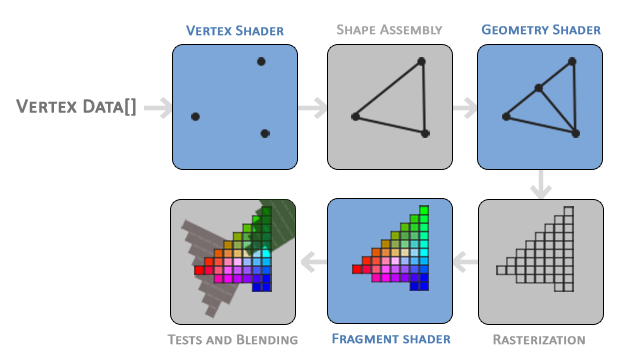
\includegraphics[scale=2]{imagenes/pipeline.png} 
	\caption{ Fases del Shader, imagen de \url{https://learnopengl.com/Getting-started/Hello-Triangle} } \label{fig:pipeline.png}
\end{figure}


\begin{figure} %con el [H] le obligamos a situar aquí la figura
	\centering
	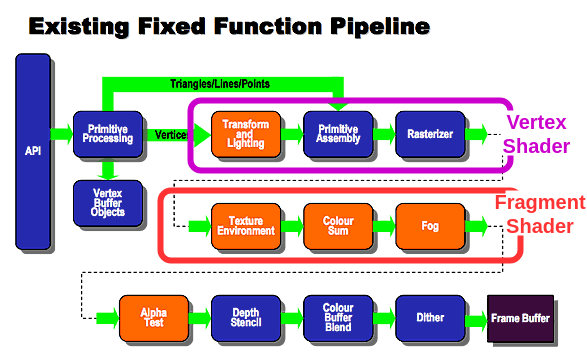
\includegraphics[scale=0.7]{imagenes/opengles_1x_pipeline.png} 
	\caption{ Flujo completo de los Shaders, imagen de \url{http://resumbrae.com/ub/dms423/18/} } \label{fig:opengles_1x_pipeline.png}
\end{figure}


Los \texttt{buffers}  son los encargados de alojar en memoria de la GPU datos para su posterior procesamiento en los Shaders, como he explicado antes. Las GPUs están especialmente diseñadas para optimizar el procesamiento en paralelo de múltiples datos con la misma función,  por ello OpenGL nos ofrece una serie de tipos de Buffers para cargar los datos en bloques grandes de forma paralela. OpenGL posee ya definidos distintos tipos para cada tipo de propósito. Los primeros son los \texttt{``Vertex Buffer Object''} (VBO), destinados a guardar vértices así como sus atributos, como pueden ser el color de cada vértice. Luego están los \texttt{``Vertex Array Object''} (VAO), son muy parecidos a los VBO, pero permiten guardar uno o muchos VBO entre otros tipos de buffers como los EBO por ejemplo. Formando así una estructura más compleja dentro de la Memoria de la GPU con toda la información relativa a un objeto. Otro tipo son los \texttt{``Element Buffer Object''} (EBO) que definen como se construye el elemento en cuestión con los vértices ya almacenados, se puede decir que definen la topología del elemento. En la figura \ref{fig:dia_buffers.png} se puede observar más claramente un ejemplo de uso de los buffers, donde los VBO se utilizan para asignarle a una figura su geometría y el color de cada vértice y el EBO se especifica los indices. Los índices son un array que contiene $n$ grupos de tres enteros, donde cada grupo indica a tres vértices, mediante la posición del array de vértices ,que componen un triángulo y $n$ es el número de triángulos que tiene el elemento. 

Es el VAO el que se manda por el el shader para generar la imagen siguiendo el esquema de la figura \ref{fig:opengles_1x_pipeline.png}.


\begin{figure} %con el [H] le obligamos a situar aquí la figura
	\centering
	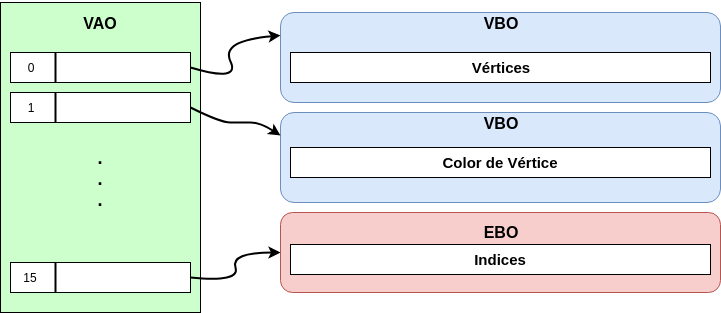
\includegraphics[scale=0.5]{imagenes/dia_buffers.png} 
	\caption{ Diagrama de funcionamiento de los Buffers VAO, VBO y EBO } \label{fig:dia_buffers.png}
\end{figure}


\subsubsection{1.1.1.2 Cámara}
La cámara es un elemento virtual en OpenGL, puesto que no existe un objeto tal y como entendemos la cámara: objeto que permite captar imágenes, pero sí se puede simular un comportamiento parecido (como nos enseñan en LearnOpenGL \cite{LearnOpenGLCamera}). OpenGL nos ofrece una serie de herramientas para esta simulación. Lo primero es que no tenemos un objeto que capte imágenes de la escena, pero si tenemos como una ``ventana'' por la cual podemos mirar. Esta ``ventana'' está en una posición fija en las coordenadas globales de la escena. Esto obliga a que para mover la cámara utilicemos la matriz de transformaciones, que es la que se aplica a todos todos los elementos en bloque. De esta forma si movemos el mundo con todos los objetos da la sensación de que la cámara se está moviendo. Por lo tanto para posicionar y que mire a donde queremos es necesario aplicar ciertas transformaciones a la matriz transformación.\\

Lo primero es posicionar la cámara en el espacio, y para ello es necesario crear una matriz con transformaciones que se añadirá a la matriz de transformación. Para posicionar la cámara se utiliza el principio de ejes de la aviación (\cite{AircraftPrincipalAxes2018}), que a su vez están basados en los ángulos de Euler (\cite{EulerAnglesWolfram}) comúnmente conocidos por ``Yaw, pitch and roll'' en la figura \ref{fig:Yaw_Axis_Corrected.png} se puede apreciar un ejemplo sobre un modelo de un avión, además de forma visual es más fácil entender en que consiste este principio. Consiste en la posición de tres ejes que hacen referencia a los ejes cartesianos en el espacio 3D, $X, Y y Z$ de esta forma es posible orientar la cámara y posicionarla donde se desee mediante la definición de los tres vectores unitarios y unas coordenadas de posición. El primer vector es el simbolizado como una $R$ y hace referencia al eje $X$ y en el modelo de Euler al eje ``Pitch'', otro vector es el vector ``Up'' simbolizado con $U$ y en el modelo de Euler llamado ``Yaw'' y por último el vector dirección, $D$, en Euler es el eje ``Roll''.\\

\begin{figure} %con el [H] le obligamos a situar aquí la figura
	\centering
	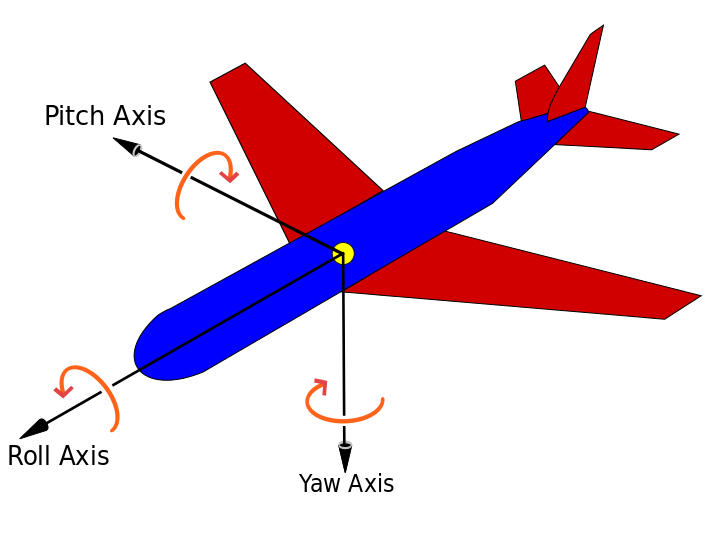
\includegraphics[scale=0.5]{imagenes/Yaw_Axis_Corrected.png} 
	\caption{ Ejes Yaw, Pitch and Roll sobre un modelo de un avión, fuente \cite{AircraftPrincipalAxes2018}} \label{fig:Yaw_Axis_Corrected.png}
\end{figure}

Combinando todos los elementos tenemos la cámara ``posicionada'' y apuntando a donde deseemos mediante la siguiente matriz de transformación que se aplicará a la matriz de transformación global. \\  
\[ 
	M=
	\begin{bmatrix}
		R_{x} & R_{y} & R_{z} & -P_{x}\\
		U_{x} & U_{y} & U_{z} & -P_{y}\\
		D_{x} & D_{y} & D_{z} & -P_{x}\\
		0 & 0 & 0 & 1 
	\end{bmatrix}
\]

Una vez tenemos la cámara posicionada y apuntando hacía donde queremos, ahora necesitamos definir otro aspecto importante de la cámara, la ``lente''. La lente de una cámara es quién le da las propiedades de cuanto capta exactamente la cámara del mundo. Igual que el objetivo de una cámara real que define el ángulo que es capaz de capturar, la calidad y la distancia máxima que es capaz de captar, en OpenGL existen propiedades que son semejantes que de encapsulan en el \texttt{frustum}. Como bien se explica en la guía de la asignatura de Informática gráfica (\cite{franciscojaviermelerorusGuiaAsignaturaInformatica2016}) el frustum es ``[...] la parte de la escena virtual que será considerada a la hora de generar la imagen 2D.'', frustum también es una forma geométrica que se obtiene cortando una pirámide de forma paralela a la base, en nuestro caso será de una base cuadrada.  Tal y como se comentó anteriormente OpenGL genera una escena virtual pero por temas de optimización no se renderiza toda ella, solo lo que se va a mostrar, por lo tanto es muy importante definir bien el frustum, ya que solo la parte de la escena que esté contenida en el frustum se renderizará. Para definir el frustum OpenGL posee los siguientes parámetros:

\begin{itemize}
	\item Near, distancia de la cámara a la cara más cercana a la cámara.
	\item Far, distancia de la cámara a la cara más lejana a la cámara.
	\item Bottom, distancia del centro de la cara a distancia Near, hasta la arista inferior del frustum.
	\item Top, distancia del centro de la cara a distancia Nea, hasta la arista superior del frustum.
	\item Right, distancia del centro de la cara a distancia Near, hasta la arista derecha del frustum.
	\item Left, distancia del centro de la cara a distancia Near, hasta la arista izquierda del frustum.
\end{itemize}

OpenGL con estos parámetros ya genera el frustum sobre la escena, se puede ver más claro en la figura \ref{fig:frustum.png}. Además al ser una escena virtual es posible modificar la perspectiva de captación de la imagen de la cámara, teniendo además de la vista en perspectiva la vista ortogonal.

\begin{figure} %con el [H] le obligamos a situar aquí la figura
	\centering
	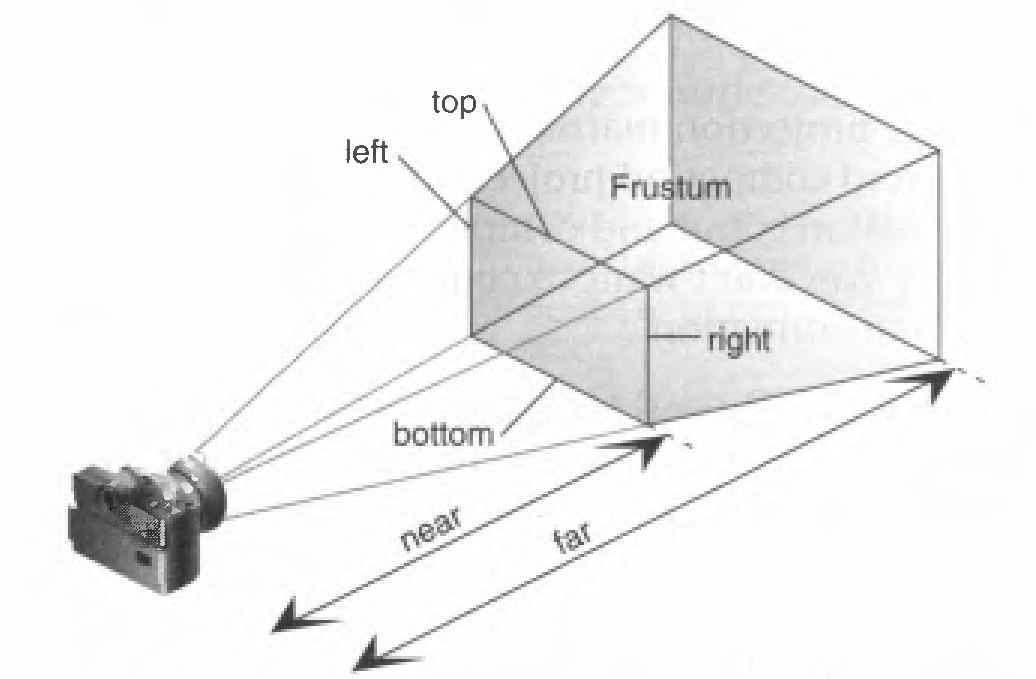
\includegraphics[scale=1]{imagenes/frustum.png} 
	\caption{ Frustum y los parámetros que los define.} \label{fig:frustum.png}
\end{figure}

\subsubsection{1.1.2 Framework de trabajo}

El proyecto se ha realizado utilizando el framework de \textit{``QT''}, en concreto, la versión \texttt{QT 5.10.1}. Se ha optado por este framework por sus elementos que ya contemplan la programación de gráficos con canvas diseñados especialmente para las API's gráficas OpenGL y Vulkan \cite{GraphicsQt11}. Además de contener una gran cantidad de clases especializadas en vectores, matrices y estructuras de datos ya implementadas. También cuenta con una gran disponibilidad independiente de la plataforma de desarrollo y la IDE de desarrollo es muy fácil de utilizar. Por estas razones se ha seleccionado \texttt{QT} como el framework de desarrollo para este proyecto.


\subsubsection{1.1.3 Entrada de Usuario}
Uno de los requisitos del sistema es la interacción con el usuario, así pues se ha decidido que el usuario pueda navegar por la escena generada para que así pueda observar completamente la malla 3D. El método de navegación consiste el movimiento de la cámara mediante el teclado. Utilizando el teclado el usuario podrá variar la posición y los elementos que definen el punto objetivo de la misma. Permitiendo que el usuario pueda elegir la vista que desee, y mejorando por consiguiente la experiencia de usuario.

\subsubsection{1.1.4 Polygon File Format (.ply)}

El formato \texttt{PLY} fué descrito por \textit{Greg Turk} en el artículo \cite{turkPLYPolygonFormat}, donde por primera vez se definía de forma pública y de forma abierta una manera de representar mallas de polígonos en ficheros de texto de forma sencilla, precisa y completa. Con este formato se puede especificar las partes de una malla que se deseen, desde solo la geometría y la topología, hasta el coeficiente de refracción. Siguiendo unas palabras reservadas y un orden se puede especificar cualquier elemento, siempre dentro del ámbito de las mallas poligonales. No es de extrañar que se haya convertido prácticamente en un estandar dentro del mundo de los gráficos, ya que al ser independiente de cualquier organismo privado no está sujeto al beneficio personal.\\

El formato de un fichero PLY sigue la siguiente estructura:

\begin{itemize}[label={--}]
	\item Cabecera: Se especifica el contenido del fichero, como su formato, número de elementos, propiedades de los elementos, etc.
	\item Lista de vértices: un listado de los vértices, en cada línea se pone un vértice. Además si se ha especificado alguna propiedad del vértice en la cabecera (como el color de vértice) se añade a continuación, el color sería en formato RGB, en la misma línea.
	\item Lista de caras: Listado que define cada una de las caras, las caras siguen el formato de indexación de vértices. Cada cara se define en un línea, así como sus posibles propiedades de cada cara.
	\item Lista de otros elementos: como pueden ser la luz ambiental que posee el objeto o cualquier otra propiedad. 
\end{itemize}

\subsection*{1.2 Procesado Geométrico}
El procesado geométrico es la segunda parte y principal del proyecto. El procesado geométrico permite la manipulación de la malla para conseguir transformarla en muchos sentidos y es un área cada vez más grande y donde más gente investiga. El procesado geométrico se puede dividir en varios campos (\cite{CS468GeometryProcessing} y \cite{GeometryProcessingCourse}).

\begin{itemize}
	\item \textbf{Captación:} consiste en generar mallas de polígonos perfectamente formadas a partir de un modelo real. En este campo se encuentran los escáneres láser, la tomografía que se usa en la sanidad y ha permitido realizar muchos avances.
	\item \textbf{Análisis:} realiza un entendimiento de la malla y la comprensión de los elementos y propiedades de la que la construyen. En la arqueología y en la ingeniería se utiliza para comprobar las propiedades físicas de los materiales mediante simulación de modelos en vez de contar con el objeto real.
	\item \textbf{Manipulación:} modifica la malla, alterando sus propiedades, la geometría, topología, etc para conseguir variaciones de la malla. En este ámbito se encuentra los modeladores 3D, que se utilizan en los videojuegos y cine, donde permiten a una figura ya creada moverle partes de forma natural sin tener que re-dibujala, también se utiliza en el estudio de objetos antiguos para la regeneración de un objeto completo a partir de partes de un objeto (\cite{meleroInteractive3DReconstruction2003}).
	
\end{itemize}

Pero el campo sobre el que trabaja este proyecto es la manipulación. Me centraré en la parte de simplificación de una malla. La simplificación de mallas es una parte importante de la manipulación, permite generar una malla parecida a la original pero con menos fidelidad y por tanto con menos elementos, dando así como resultado una malla más fácil de cargar y renderizar en vídeo. La renderización de mallas hiper realistas es un problema por el hardware actual. En el mundo de los videojuegos se exponen miles de elementos en la escena y el objetivo es que todos reaccionen en tiempo real a los eventos del jugador. Pero esto tiene un coste de computación muy elevado que a día de hoy es inasumible. Por ello se buscan métodos de mejorar el tiempo de renderizado sin que el usuario note perdida de calidad de la escena. Una de las técnicas utilizadas es el \texttt{Level Of Details}, o nivel de detalle, que consiste en tener varias mallas o modelos de un objeto con diferentes grados de calidad o exactitud con el original, de este modo se puede cargar  objetos con un tercio de los triángulos originales cuando se sitúa en el fondo de la escena y con forme nos vamos acercando al objeto se cambia por otro con más triángulos hasta llegar al modelo original. Un ejemplo gráfico es el de la figura \ref{fig:polygon-reducer-lod-1.png}, donde se ve un conejo con distintos grados de detalle y triángulos, y aunque a primera vista puede apreciarse muy claramente las diferencias si las exponemos a una cierta distancia como en la figura \ref{fig:polygon-reducer-lod-2.png} se puede ver claramente como realmente parece la misma figura.\\

Para esta técnica de reducción de triángulos se pueden aplicar distintos métodos para conseguir mallas con menos exactitud, como por ejemplo el re-modelado, donde un artista reduce los triángulos a mano o por el contrario de forma automática mediante algoritmos. En este momento entra el procesado de mallas y la simplificación geométrica. Este campo como ya se ha comentado anteriormente existen varios algoritmos que permiten reducir la cantidad de triángulos según varios criterios. En nuestro caso nos centramos en el ``decimation''.

\begin{figure} %con el [H] le obligamos a situar aquí la figura
	\centering
	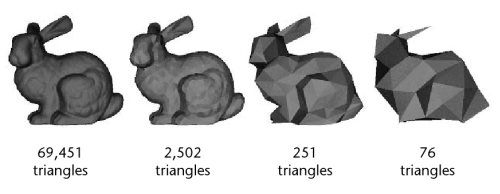
\includegraphics[scale=0.8]{imagenes/polygon-reducer-lod-1.jpg} 
	\caption{ Distintos grados de exactitud y cantidad de triángulos de una malla, fuente \url{http://polygon-reducer.pc-guru.cz/reducing-level-of-detail?skin=tisk}} \label{fig:polygon-reducer-lod-1.png}
\end{figure}

\begin{figure} %con el [H] le obligamos a situar aquí la figura
	\centering
	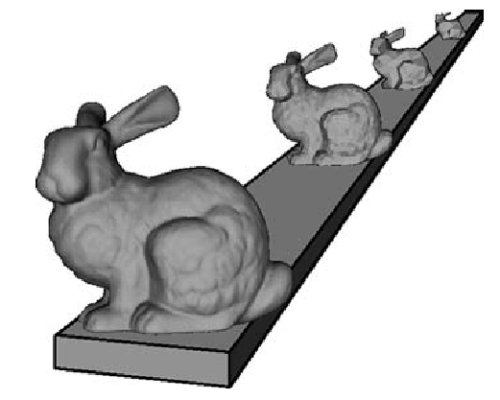
\includegraphics[scale=0.5]{imagenes/polygon-reducer-lod-2.jpg} 
	\caption{ Level of detail en práctica, fuente \url{http://polygon-reducer.pc-guru.cz/reducing-level-of-detail?skin=tisk}} \label{fig:polygon-reducer-lod-2.png}
\end{figure}

\newpage
\subsubsection*{1.2.1 Decimation}
El algoritmo de decimation (\cite{OpenMeshMeshDecimation} y \cite{mirelaben-chenCS468GeometryProcessing}) nos indica una forma de simplificar una malla para que a partir de un porcentaje de error nos genera otra malla con dicho error sobre la malla original. Entendiendo el error de una cara como la sumatoria de los ángulos que forman las normales de cara de las caras adyacentes con respecto a la normal de cara de la propia cara. En la figura \ref{fig:error_decimation.png} para calcular el error de combinar la cara $A$ y la cara $B$ tenemos la cara $A$ y la cara $B$ y para calcular el error que produce que calcular la sumatoria de los ángulos de las normales de cara de las caras $A,B,C,D,E$ y ese sería el error que se produce. De esta forma si dos caras son paralelas el error que produce al combinarlas es de $0$ pero si son perpendiculares es un error de $1.41$, siempre en radianes, en la imagen solo se muestra el ángulo $\alpha$ pero habría que calcularlo con todas las demás caras.\\


\begin{figure} %con el [H] le obligamos a situar aquí la figura
	\centering
	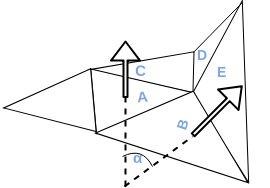
\includegraphics[scale=1]{imagenes/error_decimation.png} 
	\caption{ Ángulo que forman dos normales de cara.} \label{fig:error_decimation.png}
\end{figure}


Una vez calculado el error de combinar todas las caras con sus adyacentes, cogemos la que produce menos error y la combinamos, para combinar dos caras se utiliza el método de collapse, que explico en el siguiente apartado.\\

Existen varias formas de aplicar el método de decimation, la más usual es por aplicación incremental, es decir, se calcula la lista de caras con menos error si se combinarán y se va sacando de la lista cada elemento, se aplica el método de combinado y se actualizan los valores de la lista de errores, puesto que la combinar dos caras las caras adyacentes cambian el error que producen su combinación y posteriormente se analiza si se ha llegado a la tasa objetivo y en caso negativo se vuelve a lanzar, así hasta que se consigue la tasa objetivo.


\subsubsection{ Collapse}

La operación de colapsar dos vértices consiste en dado una semi-arista, colapsar el vértice de origen en el vértice destino. Esta operación requiere de un control de los elementos implicados pues tiene ciertas características que debe mantener. La librería de \texttt{OpenMesh} (\cite{OpenMeshBasicOperations}) se explica cómo realizar esta operación y las medidas a tener en cuenta, además de ilustrar el proceso. En la figura \ref{fig:meshcollapse.png} se puede apreciar el antes y después de aplicar el proceso de collapse a una semi-arista o a su opuesta.\\

\begin{figure} %con el [H] le obligamos a situar aquí la figura
	\centering
	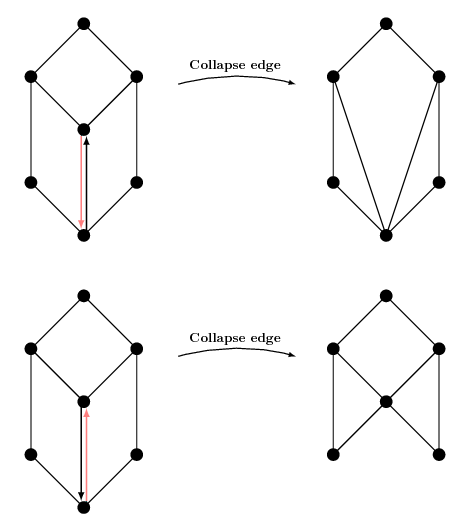
\includegraphics[scale=0.8]{imagenes/meshcollapse.png} 
	\caption{Antes de después de aplicar el método de collapse, la dirección de colapse es la semi-arista roja, fuente \url{https://www.openmesh.org/media/Documentations/OpenMesh-7.0-Documentation/a03935.html}} \label{fig:meshcollapse.png}
\end{figure}

El algoritmo de collapse, tiene que mantener la forma de la malla, es decir, que no puede crear agujeros, ni estructuras de vértices T. Tal y como de explica en la presentación sobre los problemas de las mallas de la universidad de Princeton (\cite{FrequentMeshProblems}) los vértices T (figura de un vértice T )pueden causar muchos problemas a la hora de analizar la malla o aplicarle algoritmos, el propio algoritmo de decimation o collapse requiere para un correcto funcionamiento que la malla fuente esté libre de este tipo de estructura. Los vértices T, rompen la estructura de todos los demás, pues ya no todas las caras contiene a únicamente tres vértices, si no que ahora esté número es desconocido a priori y puede variar cada vez que apliquemos una transformación. Otras características a tener en cuenta y que son altamente recomendables es que sea una malla \texttt{2-manifolds}, como se explica Daniel Müllner en  \cite{2manifoldsManifoldAtlas}, donde las caras están orientadas, no posee vértices T y la superficie no puede cortarse a sí misma. 	

\begin{figure} %con el [H] le obligamos a situar aquí la figura
	\centering
	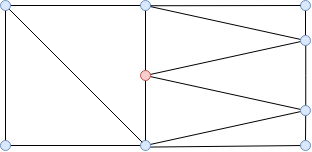
\includegraphics[scale=0.8]{imagenes/T_vertice.png} 
	\caption{Vértice T (de color rojo), frente a vértices normales (color azul)} \label{fig:T_vertice.png}
\end{figure}
%
\chapter{ Diseño}
En este capitulo vamos a tratar todo lo relacionado con el diseño del proyecto, es decir, la parte de Ingeniería del Software. Este capitulo es muy importante, ya que las decisiones aquí tomadas afectaran de forma directa a la evolución del proyecto y el desarrollo del mismo.
 
\section{Arquitectura del Software}
La arquitectura del software es una decisión muy importante, ya que establece los planos sobre los que se va a construir el software, además indica cómo se va a construir y que normas seguir. Aunque siempre se puede modificar y adaptar para los casos particulares de cada proyecto. Con esto quiero decir que la arquitectura del Software son una serie de guías y reglas para ayudarnos a construir un proyecto software correctamente pero son solo eso guías y reglas, no son una obligación y ahí es donde entra un ingeniero del software en adaptar los patrones que ya existen a un proyecto concreto o incluso en desarrollar nuevos patrones que se adapten de la mejor manera. Cada software cumple una serie de requisitos comunes con otros sistemas, pero también tiene sus peculiaridades.\\

Esta elección se ha tomado con la ayuda del libro Martin Fowler: ``patterns of enterprise application architecture'' (\cite{fowlerPatternsEnterpriseApplication2012}) donde se define que es una arquitectura software y cómo elegir un buen patrón de diseño según el sistema que se desea desarrollar. Para este caso se ha elegido el patrón de Modelo Vista Controlador, este patrón consiste en una arquitectura de capas, concretamente tres capas. Donde cada capa se encarga de una funcionalidad muy específica,  
de esta forma la funcionalidad similar está agrupada en una misma capa. El orden y la funcionalidad de las capas son:

\begin{enumerate}
	\item \textbf{Vista}: Es la capa más cercana al usuario, se encarga de la interfaz de usuario y mostrarle los eventos que ocurran. Consulta los eventos y genera la interfaz de usuario a partir de los datos que obtiene de los controladores.
	
	\item \textbf{Controlador}: Es la capa intermedia y es la más importante ya que hace de intermediaria entre los datos (Modelo) y la vista. Es la encargada de la gestión y control de los datos, así de como generar las operaciones necesarias que se mostraran en la vista así como de gestionar las entradas de usuario.
	
	\item \textbf{Modelo}: Es la capa más interna y es la encargada de gestionar los datos que utiliza el sistema. En sistemas con persistencia de datos, esta capa es la más cercana a la base de datos ya que es un reflejo de las tablas de la base de datos.
\end{enumerate}

En la figura \ref{fig:MVC-Process.png} podemos ver un diagrama de este patrón y entender mejor su funcionamiento. 

\begin{figure} %con el [H] le obligamos a situar aquí la figura
	\centering
	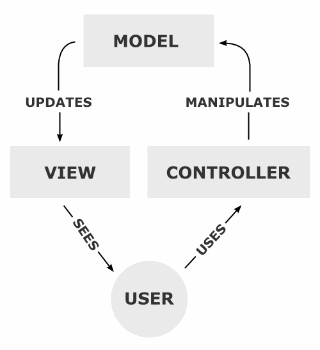
\includegraphics[scale=0.5]{imagenes/MVC-Process.png} 
	\caption{ Diagrama del patrón Modelo Vista Controlador, imagen de \url{https://es.m.wikipedia.org/wiki/Archivo:MVC-Process.png} } \label{fig:MVC-Process.png}
\end{figure}

El controlador recoge las entradas de usuario y las gestiona, en nuestro caso recogerá las pulsaciones del teclado y el movimiento del ratón que se transformarán en el movimiento de la cámara por ejemplo. El controlador será el que contenga todo el tema del procesado geométrico, el modelo contendrá las estructuras de datos para alojar los vértices, caras, semi-aristas aladas, etc. \\

\newpage
\section{ Diagrama de clases}
El diagrama de clase nos permite ver cómo se van a estructurar las clases de manera general además de ver la interacción entre ellas. El diagrama de clases se ve en la figura \ref{fig:diagramaClases.png}

\begin{figure} %con el [H] le obligamos a situar aquí la figura
	\centering
	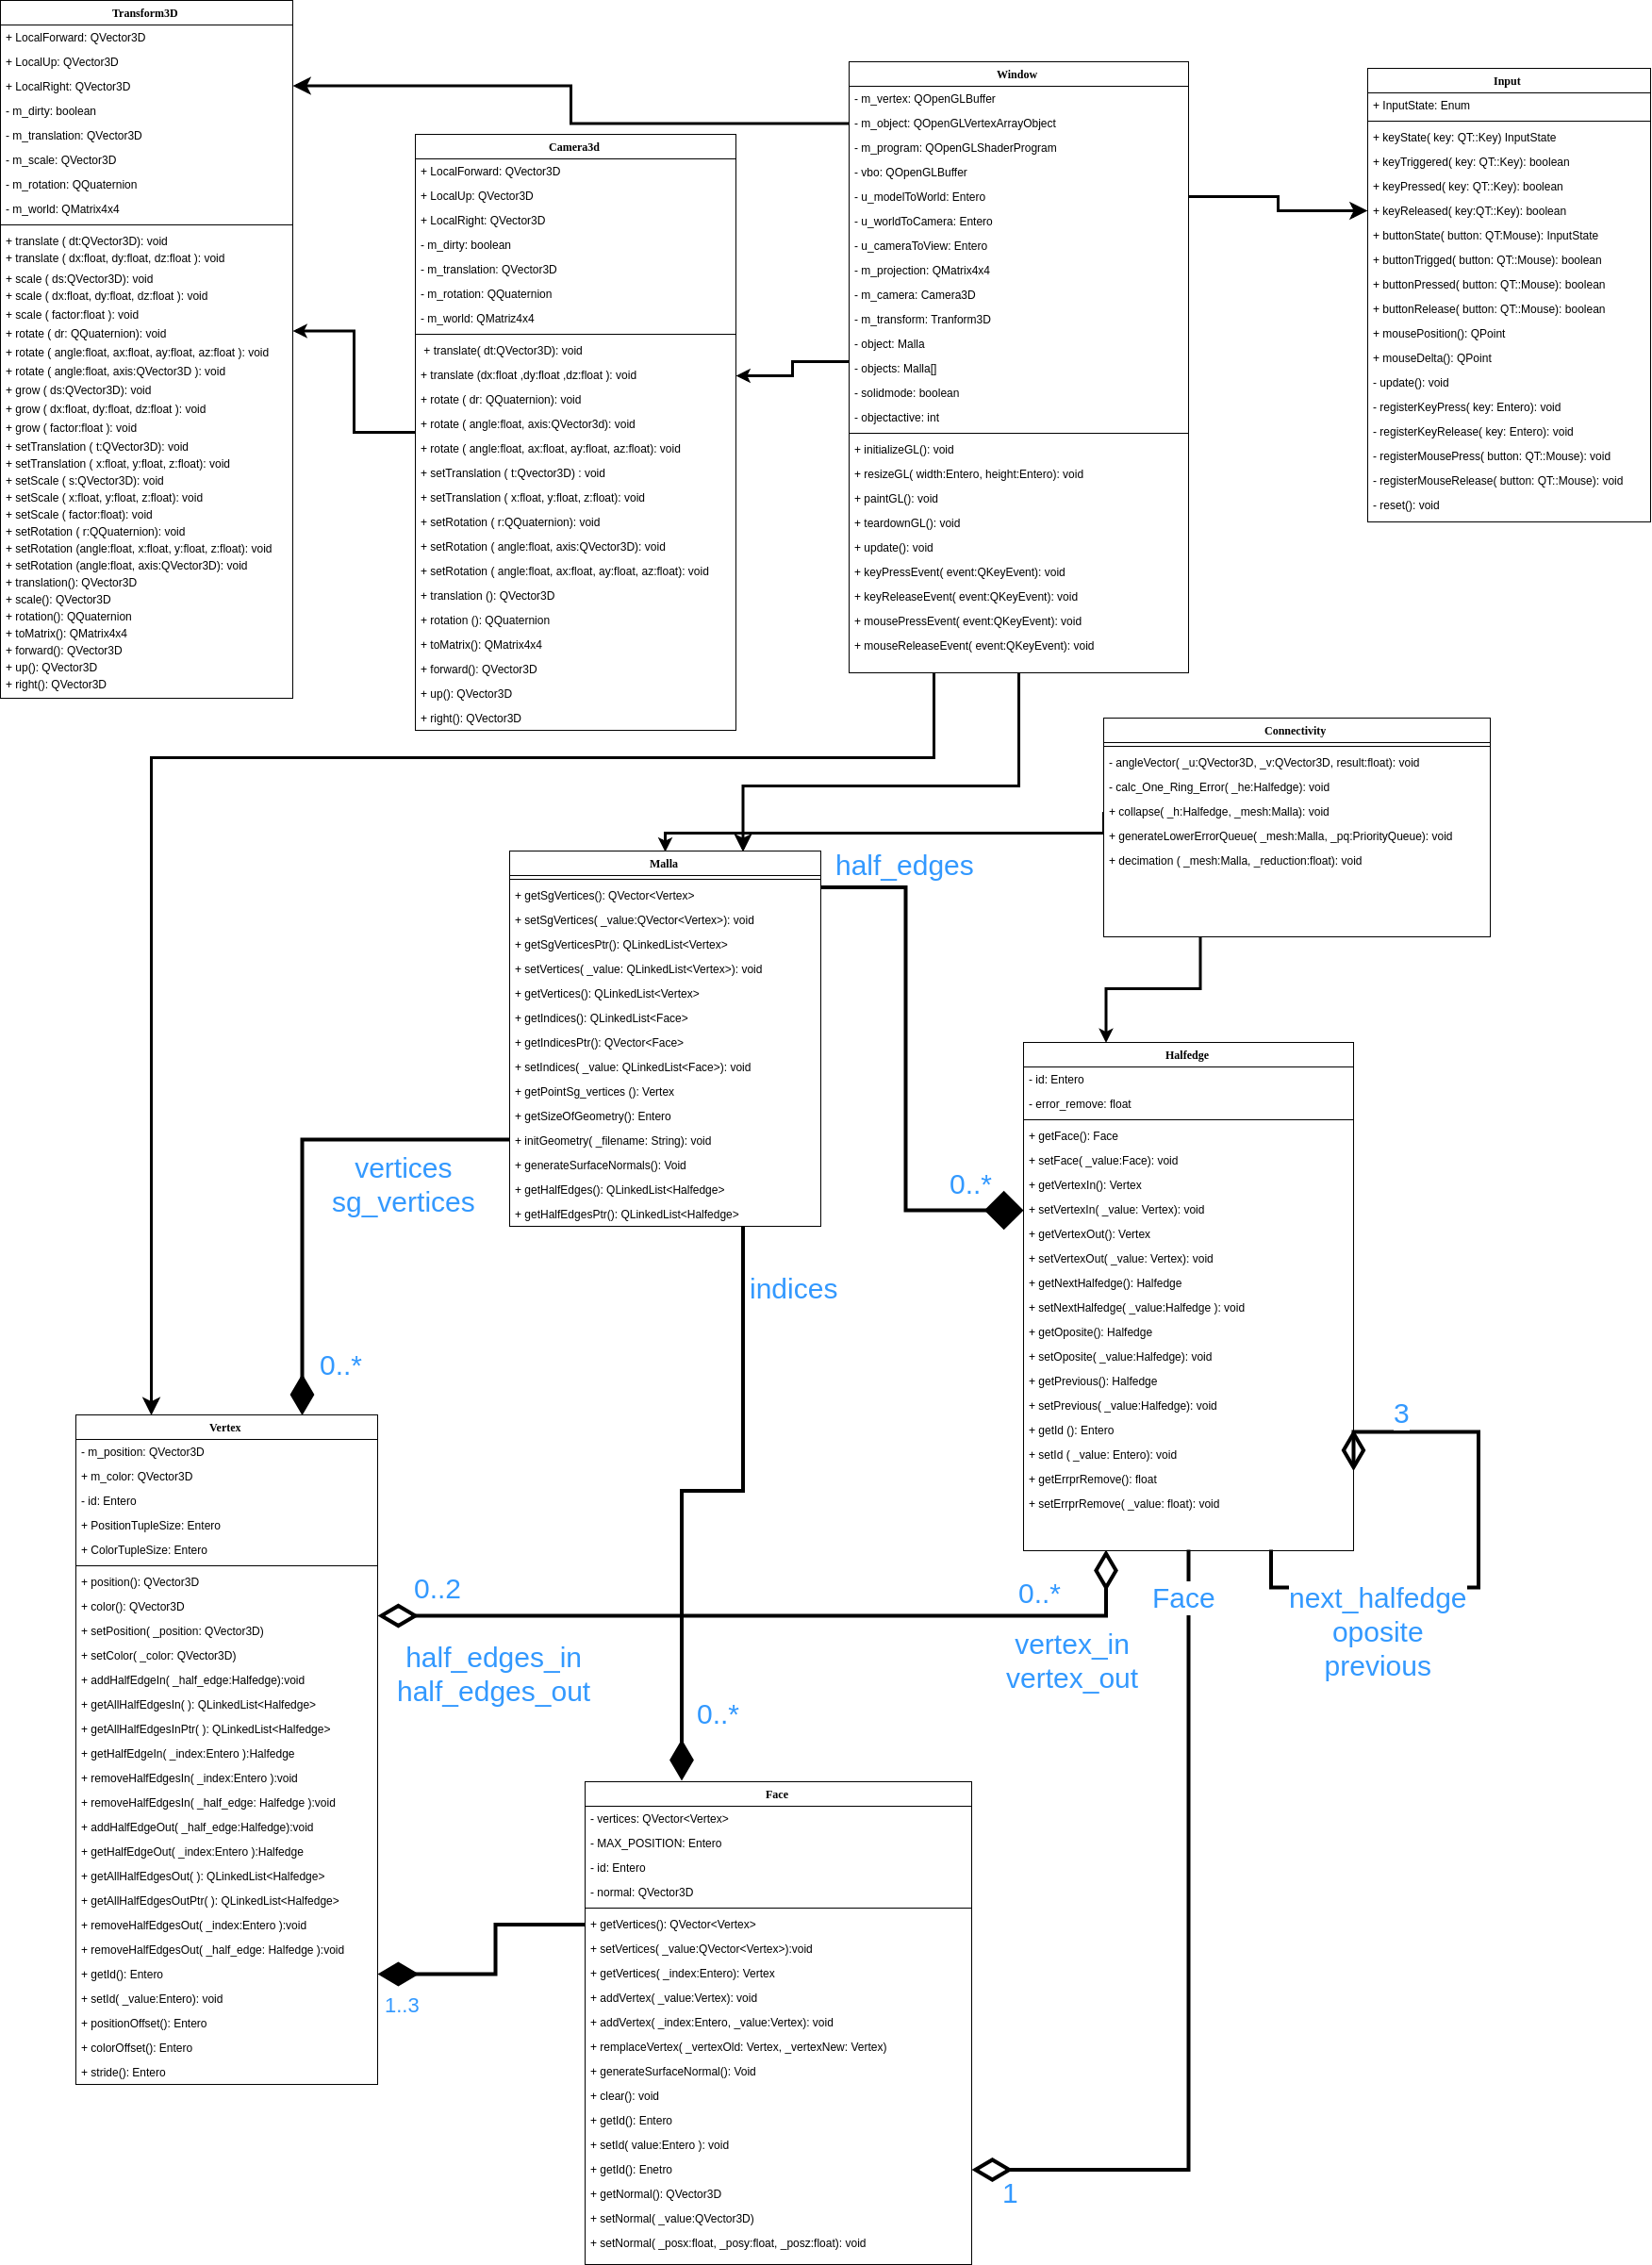
\includegraphics[scale=0.25]{imagenes/diagramaClases.png} 
	\caption{ Diagrama de clases } \label{fig:diagramaClases.png}
\end{figure}


%
\chapter{ Implementación}

\section{ Plataforma de desarrollo}
La plataforma para desarrollar la API ha sido un entorno basado en linux, concretamente\texttt{ Ubuntu 16.04LTS}. El Entorno de desarrollo elegido es \texttt{QT Creator} junto con \texttt{QT} 5.10.1. Y las librerías se apoyo son:
\begin{itemize}
	\item OpenGL 4.5.
	\item OpenMesh 7.0.
	\item CMake 3.5.1
\end{itemize} 

Además se ha utilizado un control de versiones, \texttt{git} en este caso, y para la parte de diagramas, esquemas e Ingeniería del Software la plataforma \texttt{Draw.io}. 
 
\section{ Instalación y configuración}

\subsection{ Entorno de desarrollo}
\textbf{OpenGL 4.5}
\begin{enumerate}
	\item Para conseguir la última versión de OpenGL es necesario instalar los drivers de NVidia o de ATI (según tu tarjeta gráfica), y la última versión que sea compatible con Ubuntu. Ya que los controladores de la tarjeta gráfica viene con la API de OpenGL.
\end{enumerate} 

\newpage
\textbf{QT Creator y QT 5.10.1}
\begin{enumerate}
	\item Descargar el instalador de la \href{https://www.qt.io/download}{web oficial}.
	\begin{enumerate}
		\item Ejecutar el instalador y seguir los pasos, asegurandote de marcar para instalar QTCreator (en su versión actual) y QT 5.10.1., como se ve en la figura \ref{fig:qt_install_1.png}
		\item Seleccionar la ubicación de instalación en \texttt{/usr/local/qt}.
	\end{enumerate}
\end{enumerate} 

\begin{figure} %con el [H] le obligamos a situar aquí la figura
	\centering
	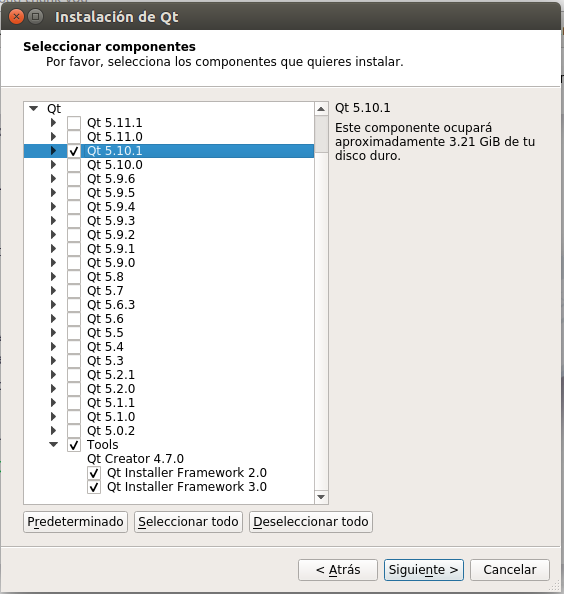
\includegraphics[scale=0.4]{imagenes/qt_install_1.png} 
	\caption{ Selección de paquetes a installar en QT installer.} \label{fig:qt_install_1.png}
\end{figure}

\textbf{OpenMesh}
\begin{enumerate}
	\item Descargar la API de OpenMesh desde \href{https://www.openmesh.org/download/}{sitio oficial}.
\end{enumerate} 	
	
	
\textbf{CMake}
\begin{enumerate}
	\item Installar CMake desde terminal y los repositorios de Ubuntu mediante el comando: \texttt{sudo apt-get install cmake}.
\end{enumerate} 



\subsection{ Configuración del Entorno}
Si has instalado QT después de tener actualizados o instalados los drivers de la tarjeta gráfica, el instalador debería de detectar que tienes instalado OpenGL e instala y configura los archivos necesarios para su funcionamiento. Además cuando se crea el proyecto con QT se debe de especificar en el archivo de configuración del proyecto (.pro) la siguiente línea:
\begin{lstlisting}[language=bash]
QT       += core gui opengl
\end{lstlisting}
para que lo compile usando la API de OpenGL.\\

Para configurar OpenMesh, es necesario tener instalado CMake, una vez comprobemos que está instalado seguimos los pasos de la documentación oficial de OpenMesh \href{URLhttps://www.openmesh.org/media/Documentations/OpenMesh-7.0-Documentation/a03933.html}{aquí}. Que nos indica según nuestro S.O. que pasos debemos seguir. Cuando se complete la configuración e instalación de OpenMesh es necesario que en el proyecto de QT en el archivo de configuración (.pro) se le indique que busqué las librerías de OpenMesh en el directorio donde lo hayamos instalado, en mi caso fue el siguiente:
\begin{lstlisting}[language=bash]
LIBS += \
/usr/local/lib/libOpenMeshCore.so  \
/usr/local/lib/libOpenMeshTools.so
\end{lstlisting}

Hay que indicar las dos librerías la \texttt{libOpenMeshCore.so} y la \texttt{libOpenMeshTools.so} ya que necesitaremos algunas de las tools que incluye, como son la lectura de ficheros PLY.

\section{ Desarrollo}

La estructura de datos es muy importante en este proyecto por ello se ha utilizado los contenedores de QT ya que viene con muchos métodos de ayuda y acceso a dichos contenedores además de traer incluidos unos iteradores para su navegación muy completos y eficientes. El contenedor principal del proyecto son las QLinkedList (\cite{QLinkedListClassQt}) ya que nos permiten una mejor gestión de la memoria y no es necesario que estén los elementos uno al lado de otro, así las eliminaciones e inserciones son muy rápidas y no afectan a las referencias que tiene unos elementos a otros puesto que cada uno siempre conserva su posición independientemente de las operaciones que se apliquen. Aunque el acceso a un elemento aleatorio es mejor con el vector y más eficiente los problemas que originan el borrado al desplazar los elementos para evitar la fragmentación interna de la memoria son mucho peores que en las listas, donde el acceso es de orden $O(n)$ pero el borrado mediante el puntero al objeto es de orden $O(1)$.

\subsection{ Input}
La clase input nos permite capturar los eventos producidos por el usuario a través del teclado y del ratón. De esta forma se le permite al usuario interactuar con la escena. La funcionalidad de esta clase es sencilla, y además cómo el tema principal del proyecto no es la interacción con el usuario, se optó por utilizar una ya creada.\\

La clase funciona como un controlador de flags, es decir, registra todas los eventos que produce el teclado y el ratón y asigna un estado a cada una de las teclas. De este modo cuando se pulsa una tecla se le asigna el flag de ``InputPressed'' y cuando se suelta pasa al flag de ``InputRelease''. Así se puede tener un control fácil de en que estado se encuentran las teclas. Para el ratón sigue la misma lógica, y además guarda la posición del puntero sobre la pantalla.

\subsection{ Camera3D}
La clase Camera3D contiene toda la lógica necesaria para crear una cámara y colocarla en la escena, como se explico en el capítulo 4, Análisis, la cámara es un factor muy importante de nuestro sistema, pero al igual que con la clase Input no es el principal tema del sistema por lo que también se optó por utilizar una ya existente, pero en ese casó si vamos a comentar los métodos más destacados así como su funcionalidad completa.\\

La clase contiene los atributos básicos de una cámara, que son: los vectores Dirección, Up y Right, además de la matriz con la rotación y traslación necesarias y por último una matriz con la transformación global del mundo. Todos estos atributos tienen sus métodos setter y getter sobrecargados para distintas opciones.\\

En cuanto a los métodos el más importante es de toMatrix(), ya que genera una matriz de proyección y restaura los flags que indican si hay alguna modificación pendiente.

\subsection{ Vertex}
Toda la lógica y modelo de los vértices se encuentra en esta clase, que posee los siguientes atributos:

\begin{itemize}
	\item \textit{m\_position: QVector3D}: representa a un vector 3D que indica la posición del vértice en el mundo de coordenadas de la escena.
	\item \textit{m\_color: QVector3D}: indica el color que posee el vértice en formáto RGB y con valor de 0 a 1. 
	
	\item \textit{halfEdgeIn: QLinkedList<HalfEdge>}: Es un conjunto de referencias a las semi-aristas que inciden sobre el vértice.
	\item \textit{halfEdgeOut: QLinkedList<HalfEdge>}: Es un conjunto de referencias a las semi-aristas que provienen del vértice.
\end{itemize}

Estos atributos son necesarios para facilitar la navegación por la malla. Poder saber qué semi-aristas salen o inciden sobre el vértice facilita mucho la gestión de las semi-aristas. Estos atributos junto con los de posición y color cuentan con los setter y getter habituales. En cuanto a los métodos principales de la clases se detallan a continuación.\\

\subsubsection*{positionOffset y colorOffset}
Indican el desplazamiento de las coordenadas de posición  y los valores de color en el objeto vértice. Cuando un objeto tiene varios atributos, estos se alojan en posiciones continuas en memoria y según el tipo de dato ocuparán más o menos posiciones. Por ejemplo el atributo posición de tipo float, ocupará 4 bytes y al ser una 3-tupla serán 12 bytes en total, tal como se refleja en el figura \ref{fig:vertex_attribute_pointer_interleaved.png}, donde se puede apreciar como las coordenadas X,Y y Z se alojan en la memoria en posiciones continuas. OpenGL provee un método para saber el offset del atributo de un objeto. Utilizando esta funcionalidad de OpenGL sabemos el offset exacto. El offset es importante  puesto que a la hora de alojar los datos en la GPU se debé indicar todos las coordenadas seguidas sin ningún dato entre medias, por ello OpenGL tiene la funcionalidad de indicarle el array de objectos y luego el offset del atributo en cuestión por si el objeto contiene más información, que suele ser lo habitual.\\

\subsubsection*{Stride}

Otro método importante requerido es el ``Stride'' que indica cuanto ocupa en memoria el objeto, para así poder saber cada cuanto espacio están separados los atributos, se puede apreciar más claramente en la figura \ref{fig:vertex_attribute_pointer_interleaved.png} con un ejemplo del array de vértices.


\begin{figure} %con el [H] le obligamos a situar aquí la figura
	\centering
	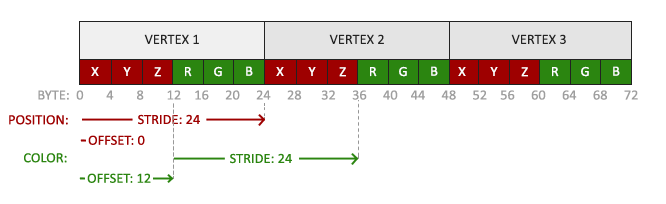
\includegraphics[scale=0.6]{imagenes/vertex_attribute_pointer_interleaved.png} 
	\caption{ Diagrama de un array de vértices, explicando gráficamente el offset y stride. Fuente de la imagen \url{https://learnopengl.com/Getting-started/Shaders}} \label{fig:vertex_attribute_pointer_interleaved.png}
\end{figure}



\subsection{ Face}
Toda la lógica y modelo de los vértices se encuentra en esta clase, que posee los siguientes atributos:

\begin{itemize}
	\item \textit{vértices: QVector<Vertex>}: representa el conjunto de vértices que forma la cara.
	\item \textit{normal: QVector3D}: vector unitario que representa la normal de la cara. Tiene el formato de 3-tupla de reales.
	\item \textit{MAX\_POSITION: Integer}: variable de control que indica el máximo número de elementos del vector vértices, así se controla que una cara o triángulo no esté formado por más de tres vértices.
\end{itemize}

Los principales métodos de esta clase se detallan a continuación.

\subsubsection*{remplaceVertex(Vertex \&\_vertexOld, Vertex \&\_vertexNew)}

RemplaceVertex pertmite dado un vértice remplazarlo por otro, para ello es necesario recorrer los vértices que forman la cara y buscar el vértice a sustituir por su atributo \texttt{id} y se sustituye.

\subsubsection*{generateSurfaceNormal}
Esta funcionalidad genera una nueva normal de cara y la asigna al atributo. Es recomendable lanzarla después de actualizar alguno de los valores del objeto, pero no se llama después de cada modificación de forma automática para que en la creación del objeto no se llame hasta que no esté totalmente creado y así dejar esta responsabilidad al programador. El método está basado en el pseudo-código de la wiki de Khronos \cite{CalculatingSurfaceNormal}.\\

El proceso para calcular la normal consiste en el siguiente proceso:\\

$$A = (x,y,z)$$ 
$$B = (x,y,z)$$ 
$$C = (x,y,z)$$
Donde $A,B,C$ son los vértices que forman la cara.
\vspace{0.3cm}
$$\overrightarrow{U} = A - B$$
$$\overrightarrow{V} = C - B$$
Obtenemos los vectores dirección $U,V$, que tiene que partir del mismo vértice (figura \ref{fig:productovectorial.png}). Ahora aplicamos el producto vectorial entre los vectores $U$ y $V$ para obtener el vector perpendicular al plano que forman. Aquí se añade una corrección respecto al algoritmo original, y es que se aumentan proporcionalmente ambos vectores, de esta forma se elimina el fallo de los decimales en el procesador, puesto que si son números muy pequeños donde los decimales son de ordenes muy bajos puede ser que con el redondeo y la discretización que aplica el ordenador se causen errores considerables.
Ahora si se puede aplicar el producto vectorial.
\begin{figure} %con el [H] le obligamos a situar aquí la figura
	\centering
	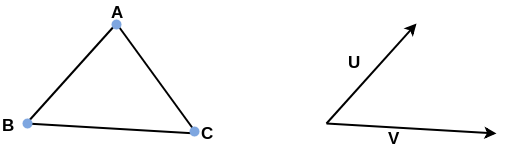
\includegraphics[scale=0.4]{imagenes/productovectorial.png} 
	\caption{Resultado de Restar los Vértices A - B y C - B} \label{fig:productovectorial.png}
\end{figure}

\[ 
N = \overrightarrow{U} \times \overrightarrow{V} = \begin{bmatrix}
i & j & k \\
U_x & U_y & U_z \\
V_x & V_y & V_z 
\end{bmatrix}  
\]

\vspace{0.3cm}

$$\overrightarrow{N_x} = \overrightarrow{U_y}*\overrightarrow{V_z} - (\overrightarrow{U_z}*\overrightarrow{V_y})$$
$$\overrightarrow{N_y} = \overrightarrow{U_z}*\overrightarrow{V_x} - (\overrightarrow{U_x}*\overrightarrow{V_z})$$
$$\overrightarrow{N_z} = \overrightarrow{U_x}*\overrightarrow{V_y} - (\overrightarrow{U_y}*\overrightarrow{V_x})$$

Ahora es necesario aplicar una normalización del vector normal. Esto se realiza mediante la división del módulo unidad del vector.

$$ ||N|| = \sqrt{N_x^2 + N_y^2 + N_z^2}$$

\begin{center}
$ N_x = \frac{N_x}{||N||}$
$ N_y = \frac{N_y}{||N||}$
$ N_z = \frac{N_z}{||N||}$
\end{center}


Una vez normalizado. Hay que ajustar los ejes por si alguna coordenada esta en negativo que es normal en el mundo 3D, pero en el vector de cara tiene que ser positivo. Así pues se calcula la normal de cara.

\newpage
\subsection{ HalfEdge}
Es una de las clases más importantes del proyecto, ya que alberga una de las funcionalidades más importante. Los atributos que la define, son muy parecidos a los descritos anteriormente:

\begin{itemize}
	\item \textit{vertexIn: Vertex}: referencia al vértice sobre el que incide la semi-arista.
	\item \textit{vertexOut: Vertex}: referencia al vértice del que proviene la semi-arista.
	\item \textit{face: Face}: una referencia a la cara adyacente, o que está formada en parte por la semi-arista.
	\item \textit{next: HalfEdge}: referencia a la semi-arista siguiente.
	\item \textit{previous: HalfEdge}: referencia a la semi-arista anterior.
	\item \textit{oposite: HalfEdge}: referencia a la semi-arista opuesta.
	\item \textit{errorRemove: Float}: indica el valor del error que produce si se elimina la semi-arista.
\end{itemize}

Los métodos de la clase son los típicos setter y getter, ya que esta clase cumple completamente con el patrón MVC y con su categoría de modelo.

\subsection{ Malla}
La clase malla es otra de las clases más importante del proyecto ya que contiene toda la lógica de la malla de triángulos. Los atributos que forman esta clase son:

\begin{itemize}
	\item \textit{vertices: QLinkedList<Vertex>}: un array de referencias a los vértices que componen la malla.
	\item \textit{sg\_vertices: QVector<Vertex>}: es un array de referencias ordenado de los vértices de la malla. Cada tres vértices indican las caras.
	\item \textit{indices: QLinkedList<Face>}: un conjunto de referencias a las caras que forman la malla.
	\item \textit{half\_edges:  QLinkedList<HalfEdge>}: conjunto de referencias a las semi-aristas que forman la malla.
\end{itemize}

Aunque los atributos sean pocos la organización del proyecto en distintas clases y métodos ha facilitado la composición de esta clase. Además el único atributo un poco más especial es el \textit{sg\_vertices} el cual contiene una referencia a los vértices ordenados para formar la malla. Esto es así para poder pasarle este vector de vértices a OpenGL y que el genere la malla. OpenGL tiene que recibir como parámetro un listado de vértices ordenados de tres en tres para generar las caras. En la figura \ref{fig:sgvertices.png} se puede observar cómo se colocan los vértices en dicho array para su correcta interpretación por parte de OpenGL. Es cierto que esta forma requiere más memoria que otras analizadas, pero con los equipos actuales, la utilización de referencias y la optimización de OpenGL a la hora de colocar los datos en las GPU se ha considerado que es una buena opción para nuestro caso. Además de los típicos setter y getter para todas las colecciones de objetos cabe destacar los siguientes métodos:\\

\begin{figure} %con el [H] le obligamos a situar aquí la figura
	\centering
	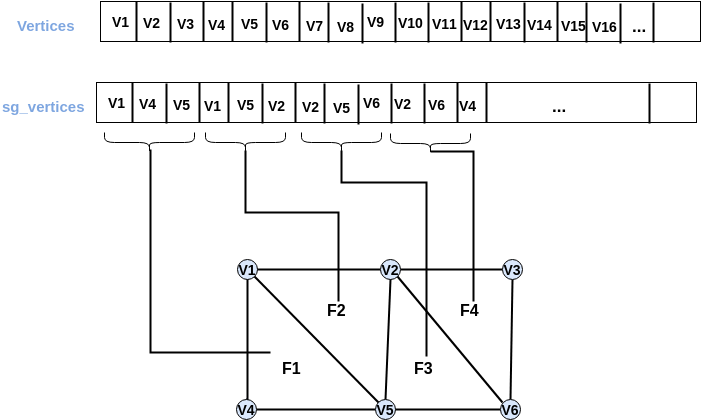
\includegraphics[scale=0.4]{imagenes/sgvertices.png} 
	\caption{Esquema de funcionamiento del atributo sg\_vertices conforme a lo establecido en OpenGL} \label{fig:sgvertices.png}
\end{figure}

\subsubsection*{initGeometry(string \_filename)}

La principal funcionalidad de este método es la de cargar una malla PLY en la estructura de datos interna. Para ello se hace uso de la API de OpenMesh, que nos permite leer un fichero PLY y cargarlo en su estructura de datos propia. Ahora la complejidad es pasar de la estructura de datos de OpenMesh a la propia, ya que la de OpenMesh utiliza muchos atributos más que no son requeridos para el proyecto y por tanto es espacio que conseguimos ahorrar. El proceso detallado es el siguiente:

\begin{enumerate}
	\item Cargar los vértices, OpenMesh contiene los vértices mediante una clase Handler y que se accede a través de iteradores. Una vez tenemos los iteradores consultamos la malla de OpenMesh solicitándole el vértice que apunta el iterador. Ya solo falta guardarlo en nuestro array particular de vértices.
	
	\item Cargar las caras, las caras son una secuencia de las posiciones de los vértices en grupos de tres que indican qué vértices forman la cara. Así pues la forma de conseguir esta secuencia se realiza mediante el id. Cada vértice añadido se le ha dado un id, que es un número desde el 0 hasta el número de vértices totales, de esta forma el vértice 0, tiene el id 0, y el vértice n, tiene el id n. Esto se cumple para el estado inicial, si se produce alguna alteración en el vector de vértices esta regla ya no se garantiza, pero para este caso sí. Entonces se recorre el listado de caras de OpenMesh y luego dentro de cada cara se coge el vértice de nuestro array con en la posición que marca los indices de la cara de OpenMesh.\\
	
	Además en este momento se calcula la normal de cara conforme de crea la cara en mi estructura.
	
	\item Semi-aristas aladas, las semi-aristas del mismo modo que los elementos anteriores se les asigna un id al crearlos y también están guardados en clases handler pero en este caso las semi-aristas contiene mucha información de los elementos anteriores, vértices y caras. Para ello se repite el proceso de recorrerlas con los iteradores y sacar la información deseada. A continuación se obtiene las caras mediante los métodos que nos provee OpenMesh que nos permiten consultar la posición de la cara mediante el iterador de la semi-aristas, así que aprovechando la propiedad descrita anteriormente de los id, se inicializa la cara incidente, los vértices sobre el que incide la semi-arista y el vértice del que parte.\\
	
	Por último una vez guardadas todas las semi-aristas se procede a asignar las semi-aristas de referencia, la siguiente, la anterior y la posterior. Volviendo a aprovechar la propiedad de los id pero esta vez con las semi-aristas, ya que OpenMesh nos vuelve a indicar las referencias mediante los ids.
	
	\item Como último paso es generar la geometría de la malla, esto se realiza con el método de generateGeometry.
	 
\end{enumerate}

\subsubsection*{generateGeometry}
Genera la geometría de la malla mediante la inicialización del vector sg\_vertices. Para ello recorro el listado de caras y dentro de cada cara se recorre el listado de sus tres vértices. Ahora solo hay que añadir los vértices en el vector de sg\_vertices. De esta forma simple se inicializa el vector.


\subsection{Connectivity}

La clase Connectivity no posee atributos como tal, ya que es la encargada de encapsular los algoritmos de procesado geométrico, por ello suelen recibir como parámetro la malla sobre la que aplicar el algoritmo y otros parámetros de configuración.

\subsubsection*{angleVector( u, v, resultado)}
La funcionalidad de este método es la de calcular el ángulo que forman los vectores $U$ y $V$ y guardar el resultado en la variable ``resultado''. Básicamente el método realiza un producto cruzado para obtener el angulo en radianes. Si el resultado fuera una indeterminación se aplica un valor alto.

\subsubsection*{calcOneRingError( halfedge)}
Método que calcula el error que produciría si se eliminase la arista pasada por parámetro. Realiza dicho cálculo y lo asigna al atributo de la semi-arista. El cálculo de error de un anillo de distancia se explicó en el capitulo 4, Análisis, y se ha implementado tal y como se espera.

\newpage
\subsubsection*{collapse (halfedge, Malla)}
Es uno de los métodos principales del proyecto y realiza una simplificación de una arista, junto con las dos caras a la que delimita y el vértice origen de la misma. La semi-arista dada como parámetro define la dirección y que vértice se colapsa con quién, mediante los atributos \textit{vertexIn} y \textit{vertexOut}. El proceso de collapse se define por el siguiente pseudo-código:

\begin{lstlisting}[frame=single]
h = semi-arista a eliminar;
hn = semi-arista siguiente a h;
hp = semi-arista anterior a h;

o = semi-arista opuesta a h;
on = semi-arista siguiente a o;
op = semi-arista anterior a o;

vh = vertice sobre el que incide h;
vo = vertice origen de h;

mesh.eliminaCara(h.getCara());
mesh.eliminaCara(o.getCara());

// Re-estructuracion de las referencias de las semi-aristas opuestas de las caras eliminadas.
hn.getOposite().getOposite() = hp.getOposite();
hp.getOposite().getOposite() = hn.getOposite();

on.getOposite().getOposite() = op.getOposite();
op.getOposite().getOposite() = on.getOposite();

// Eliminar las referencias a las semi-aristas en los vertices
hn.getVertexIn().removeHalfEdge(hn);
hn.getVertexOut().removeHalfEdge(hn);

hp.getVertexIn().removeHalfEdge(hp);
hp.getVertexOut().removeHalfEdge(hp);

h.getVertexIn().removeHalfEdge(h);
h.getVertexOut().removeHalfEdge(h);

on.getVertexIn().removeHalfEdge(on);
on.getVertexOut().removeHalfEdge(on);

op.getVertexIn().removeHalfEdge(op);
op.getVertexOut().removeHalfEdge(op);

o.getVertexIn().removeHalfEdge(o);
o.getVertexOut().removeHalfEdge(o);

mesh.remove(hn,hp,on,op);

// Las semi-aristas que inciden sobre vo ahora inciden sobre vh
for(HalfEdge he: vo.AllHalfEdgeIn){
	he.setVertexIn(vo);
	vh.addHalfEdgeIn(he);
}

// Las semi-aristas que tiene origen sobre vo ahora lo tienen sobre vh
for(HalfEdge he: vo.AllHalfEdgeOut){
	he.setVertexIn(vo);
	vh.addHalfEdgeIn(he);
}

mesh.getCaras.remplazar(vo,vh);
mesh.getCaras.recalcularNormaldeCaras();

mesh.getAllHalfEdges.remove(h,o);
mesh.getAllVertices.remove(vo);

\end{lstlisting}

De la línea 16 a la línea 20 se realiza una re-estructuración muy importante para la continuidad de la malla. Esta parte del proceso es delicada ya que requiere que las caras que se van a eliminar mantengan las propiedades en el resto por lo tanto se aplica que la semi-aristas opuestas que se van a eliminar se enlacen con las semi-aristas opuestas de las semi-aristas siguientes. Para entenderlo de forma más fácil ver la figura \ref{fig:collapse_011.png}, donde las semi-aristas opuestas a hn y hp son hn.O y hp.O respectivamente. Después de eliminar las caras 0 y 1, las opuestas de hn.O y hp.O estarán apuntando a posiciones vacías y por tanto ya no se mantendrían las propiedades de la malla. Así que se asignan las hn.O y hp.O como opuestas entre sí manteniendo la concordancia entre caras.

\begin{figure} %con el [H] le obligamos a situar aquí la figura
	\centering
	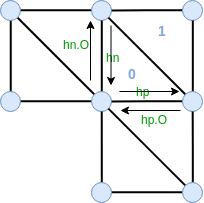
\includegraphics[scale=0.8]{imagenes/collapse_011.png} 
	\caption{Esquema de re-estructuración de semi-aristas opuestas en el método collapse. En Azul las caras y en Verde las semi-aristas.} \label{fig:collapse_011.png}
\end{figure}

\newpage
\subsubsection*{generateLowerErrorQueue( Malla, PriorityQueue)}

Este es otro de los métodos fundamentales del procesado geométrico ya que nos define una cola con prioridad de todas las semi-aristas de la malla de triángulos. La lógica de este método es la siguiente:

\begin{lstlisting}[frame=single]
priorityQueue.clear;

for(HalfEdge he: malla.getAllHalfEdges){
	calcOneRingError(he);
	priorityQueue.add(he);
}

\end{lstlisting}

Al crear una estructura de datos con bastante funcionalidad y encapsular los métodos la construcción de este método es más lógica que compleja.

\subsubsection*{decimation( Malla, tasaReducción)}
Y por último el método más importante del proyecto, donde se realiza la simplificación iterativa del collapse. Este método es el que enlaza toda la funcionalidad anterior y completa un flujo del proceso.
La lógica que sigue es la siguiente:

\begin{lstlisting}[frame=single]
num_reducciones = calcularNumeroReducciones(tasaReduccion);

generateLowerErrorQueue(pq);
HalfEdge he;

for(i=0 hasta num_reducciones){
	he = malla.getHalfEdge(pq.top());
	
	if(he.getFace != he.getOposite.getFace)
		collapse(he,malla);
	else
		mostrar error;
	
	pq.pop
	
	//Actualizamos los valores
	generateLowerErrorQueue(pq);
	
}
\end{lstlisting}

De esta forma el método de \textit{decimation} va reduciendo arista a arista hasta llegar a la tasa de reducción elegida y siempre reduciendo la arista que menos error produce, obteniendo así una malla optima en todo momento.
%
\chapter{ Pruebas}

\section{ Decimation}
En este capitulo solo se realizarán pruebas del método decimation puesto que ya realiza internamente uso de los demás métodos y genera el objetivo final del proyecto. Por tanto se analizarán los resultados de las pruebas obtenidas de la ejecución del método sobre tres mallas ply:
\begin{itemize}
	\item \textbf{sphere:} Contiene 840 caras y 422 vértices y se ve como en la figura \ref{fig:esfera_100.png}.
	\item \textbf{beethoven:} Contiene 5030 caras y 2521 vértices y se ve como en la figura \ref{fig:beethoven_100.png}.
	\item \textbf{big\_dodge:} Contiene 16646 caras y 8477 vértices y se ve como en la figura \ref{fig:coche_100.png}.
\end{itemize} 

\begin{figure} %con el [H] le obligamos a situar aquí la figura
	\centering
	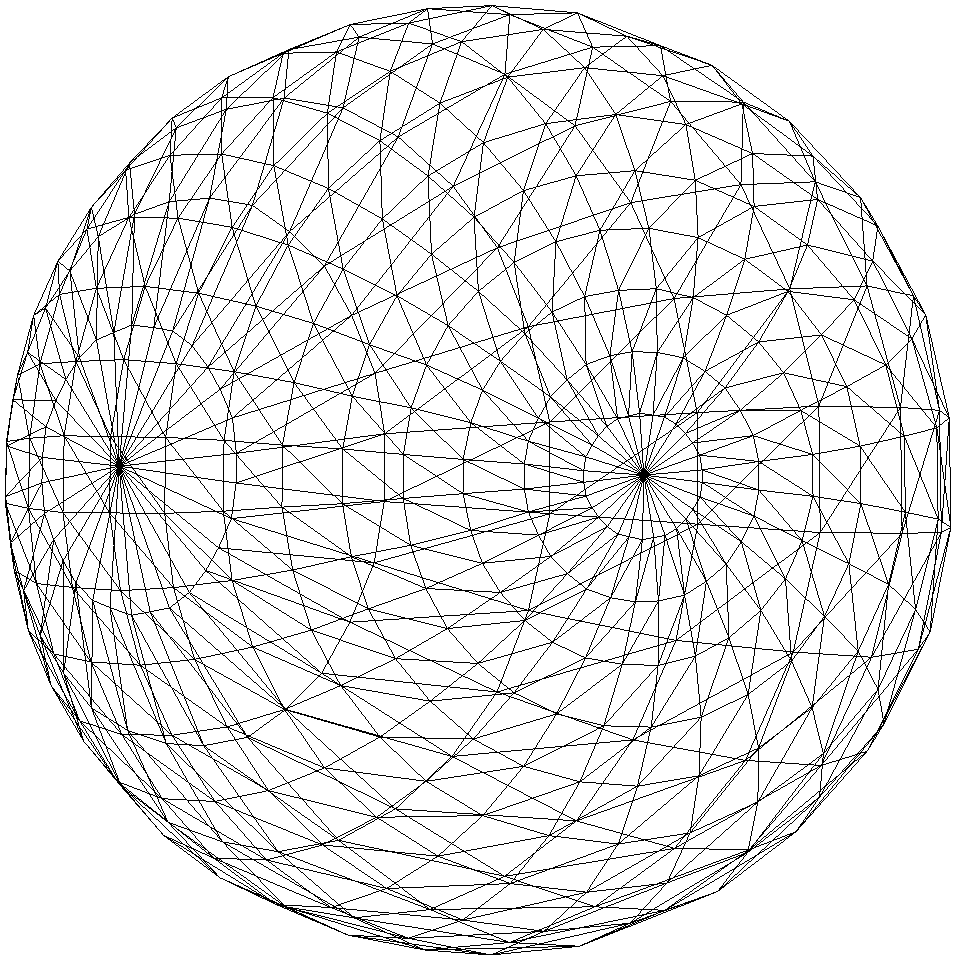
\includegraphics[scale=0.25]{imagenes/esfera_100.png} 
	\caption{Malla sphere.ply original.} \label{fig:esfera_100.png}
\end{figure}

\begin{figure} %con el [H] le obligamos a situar aquí la figura
	\centering
	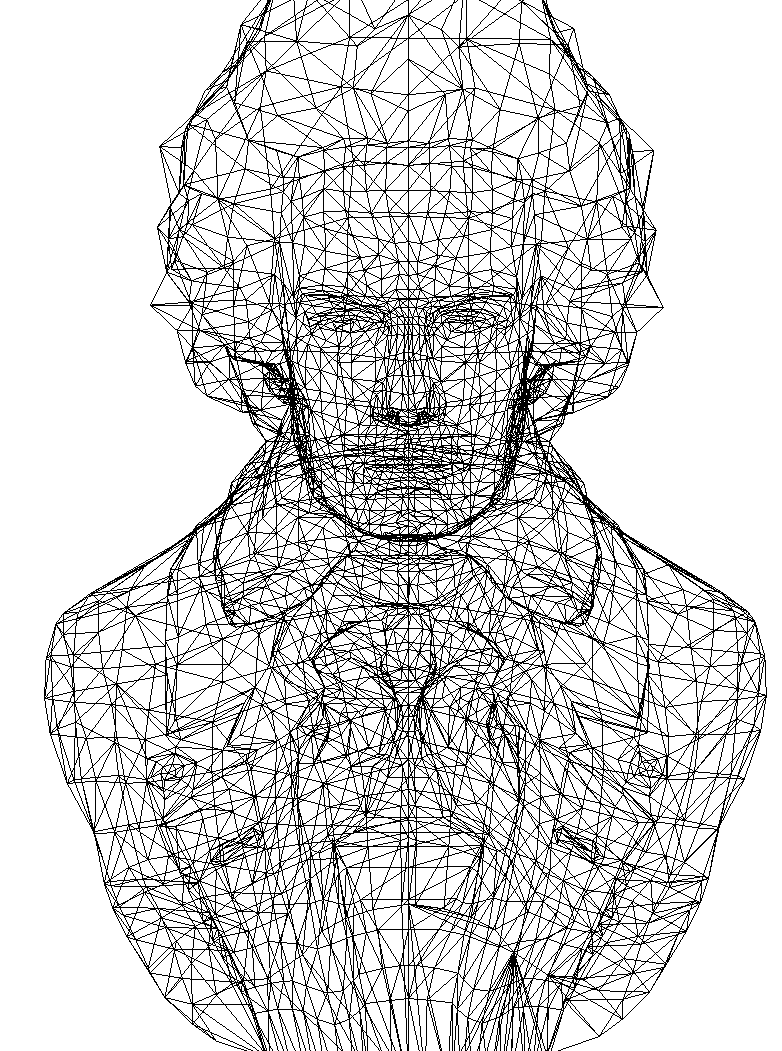
\includegraphics[scale=0.3]{imagenes/beethoven_100.png} 
	\caption{Malla beethoven.ply original.} \label{fig:beethoven_100.png}
\end{figure}

\begin{figure} %con el [H] le obligamos a situar aquí la figura
	\centering
	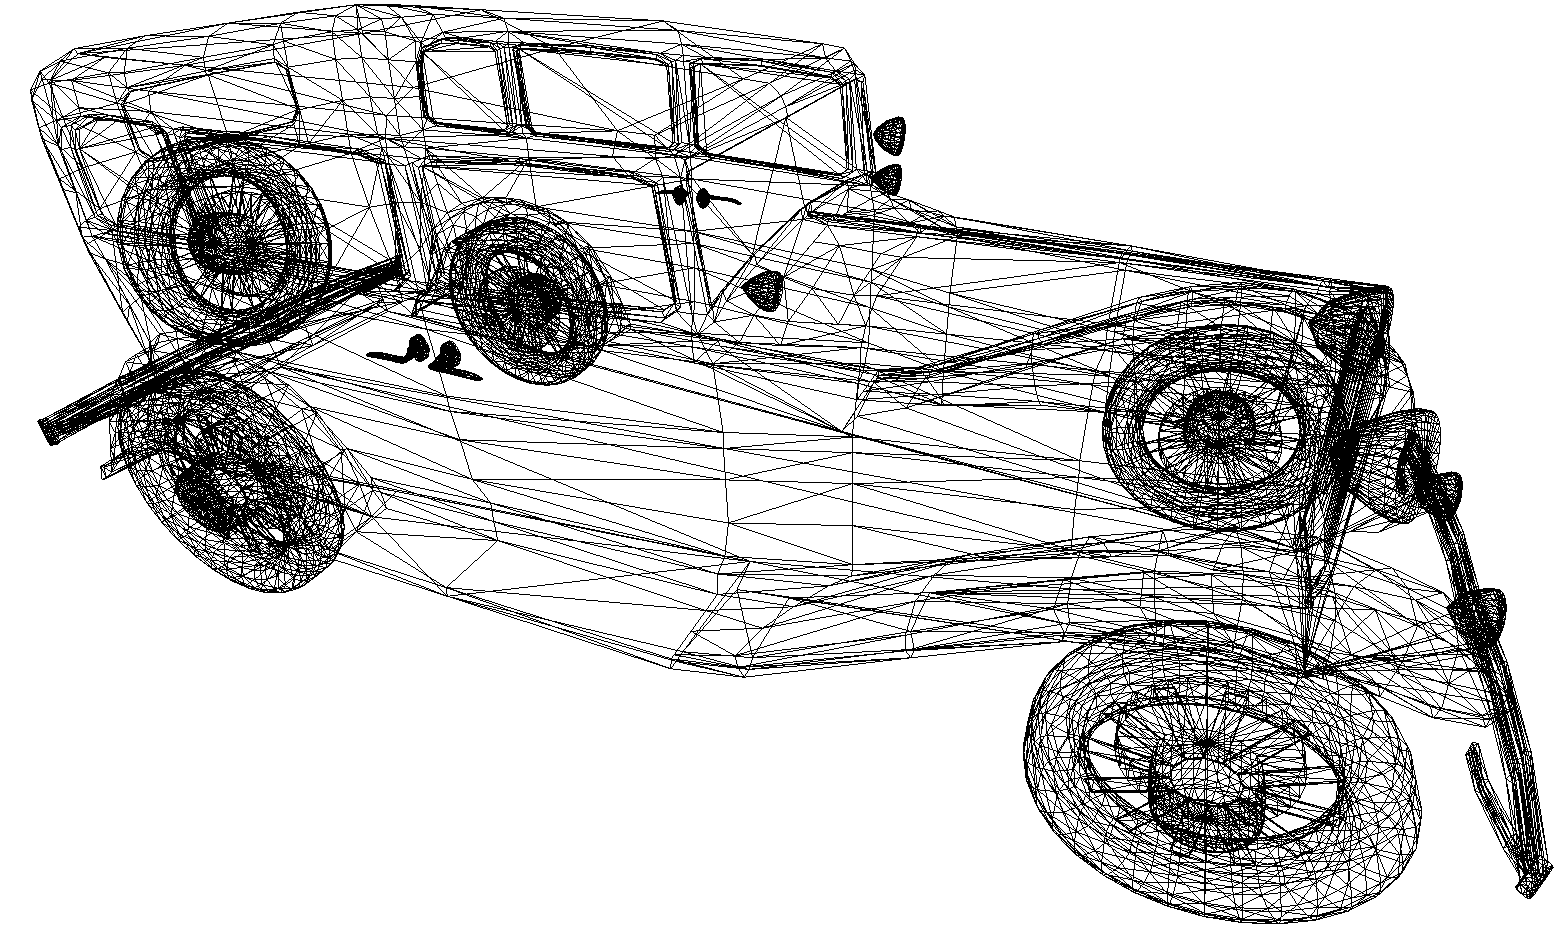
\includegraphics[scale=0.2]{imagenes/coche_100.png} 
	\caption{Malla big\_dodge.ply original.} \label{fig:coche_100.png}
\end{figure}

A estas mallas se les ha aplicado una tasa de reducción del 90\%, 75\%, 50\% y 25\%, y en cada tasa se ha obtenido el tiempo de computo del método \textit{decimation} y el número de caras obtenidas después de su aplicación. Todas las capturas de este capítulo se adjuntan a la memoria en la carpeta ``capturas'' con su resolución original. La tasa de reducción significa que la malla destino es ese porcentaje menos exacta a la original. Un ejemplo es una tasa de reducción al 90\% significa que la malla resultante tendrá un 10\% de error con respecto a la original y por tanto tendrá un 90\% menos de caras.

\newpage
\subsection{Sphere} 
Los resultados para la malla de Sphere que contiene una esfera han sido los siguientes.\\

Como se puede apreciar en la figura \ref{fig:esfera_90.png} donde solo se ha aplicado una tasa de reducción al 90\% la figura apenas se aprecia cambios significativos. Donde más se pueden apreciar la simplificación es en las tapas superior e inferior, aunque en la imagen de ven al frente y en la parte de atrás.\\ 

\begin{figure} %con el [H] le obligamos a situar aquí la figura
	\centering
	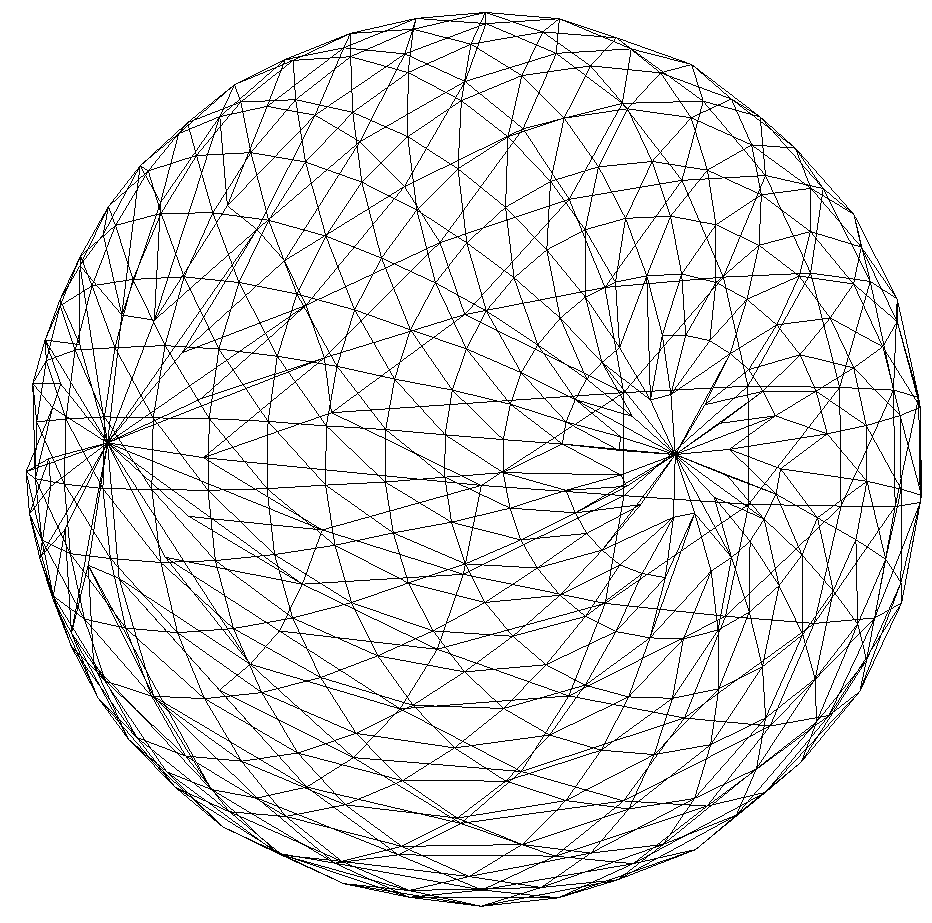
\includegraphics[scale=0.25]{imagenes/esfera_90.png} 
	\caption{Malla sphere.ply con una tasa de reducción del 90\%.} \label{fig:esfera_90.png}
\end{figure}

Si aplicamos ahora una tasa de reducción al 75\%, figura \ref{fig:esfera_75.png}, ya se puede apreciar cómo se empieza a deformar la esfera para ser más irregular, pero sigue manteniendo la silueta. Otro factor que se puede apreciar es que las primeras caras que se simplifican son las que forman las tapaderas superior e inferior, es decir, donde hay más caras pero más pequeñas que forman una superficie más homogénea al resto, con lo que se comprueba que el método simplifica primero las caras con que menor error van a producir.\\

\begin{figure} %con el [H] le obligamos a situar aquí la figura
	\centering
	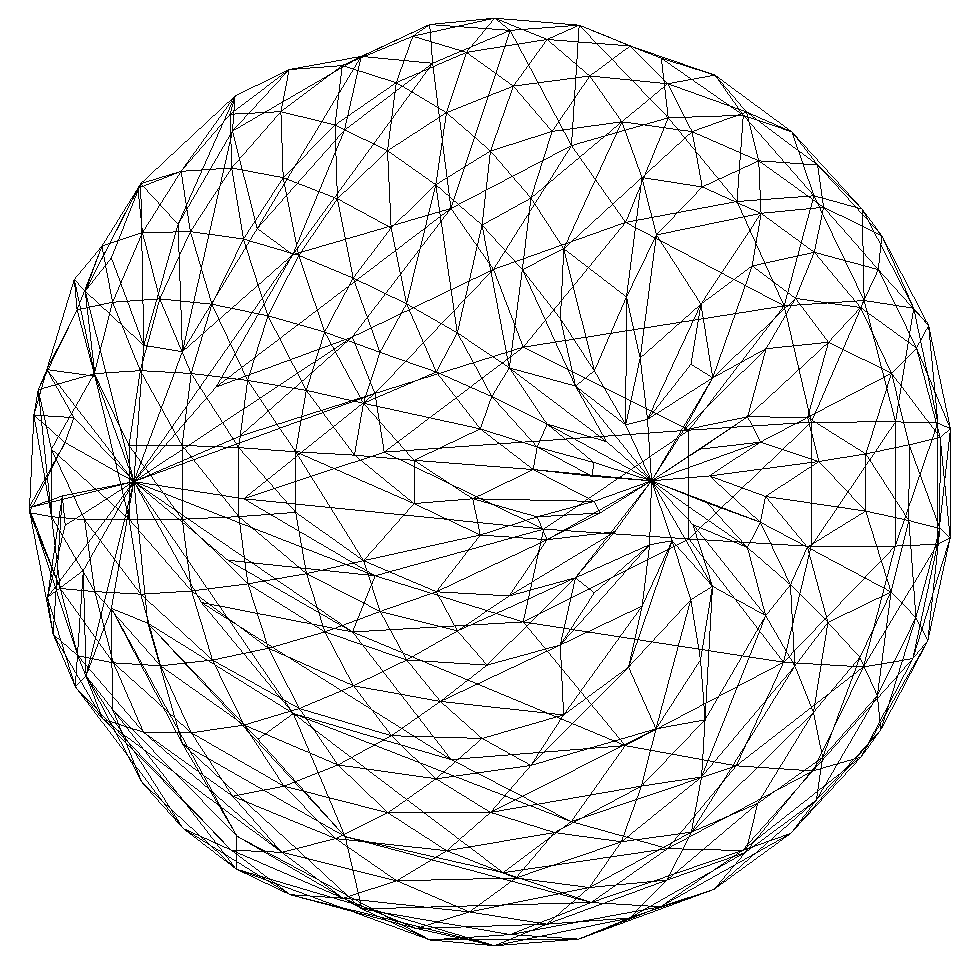
\includegraphics[scale=0.25]{imagenes/esfera_75.png} 
	\caption{Malla sphere.ply con una tasa de reducción del 75\%.} \label{fig:esfera_75.png}
\end{figure}

Aplicando una tasa de reducción más restrictiva al 50\%, figura \ref{fig:esfera_50.png}, ya la forma se compromete y aunque sigue manteniendo una silueta similar a una esfera. Las tapas superior e inferior ya han perdido su curvatura y pasan a ser lisas.\\

\begin{figure} %con el [H] le obligamos a situar aquí la figura
	\centering
	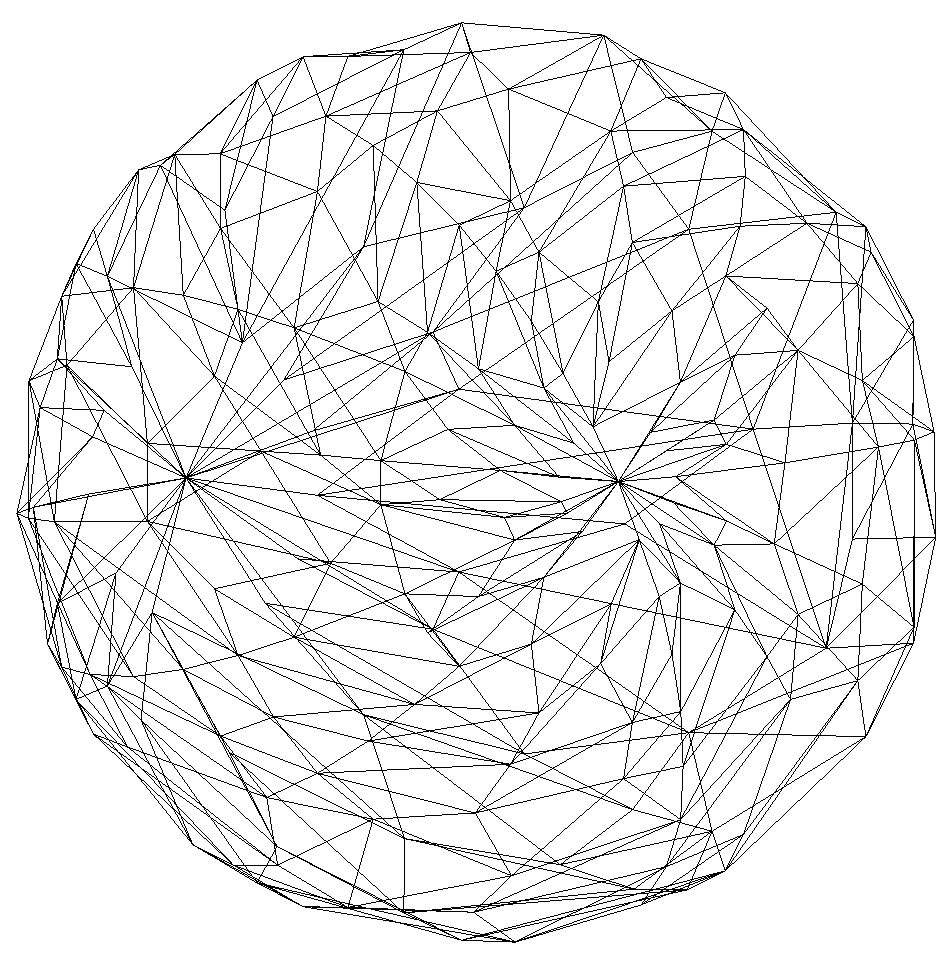
\includegraphics[scale=0.25]{imagenes/esfera_50.png} 
	\caption{Malla sphere.ply con una tasa de reducción del 50\%.} \label{fig:esfera_50.png}
\end{figure}

Con la tasa de reducción al 25\%, figura \ref{fig:esfera_25.png}, conseguimos una gran reducción en el número de caras, pero cuesta observar la similitud con una esfera perfectamente redonda.

\begin{figure} %con el [H] le obligamos a situar aquí la figura
	\centering
	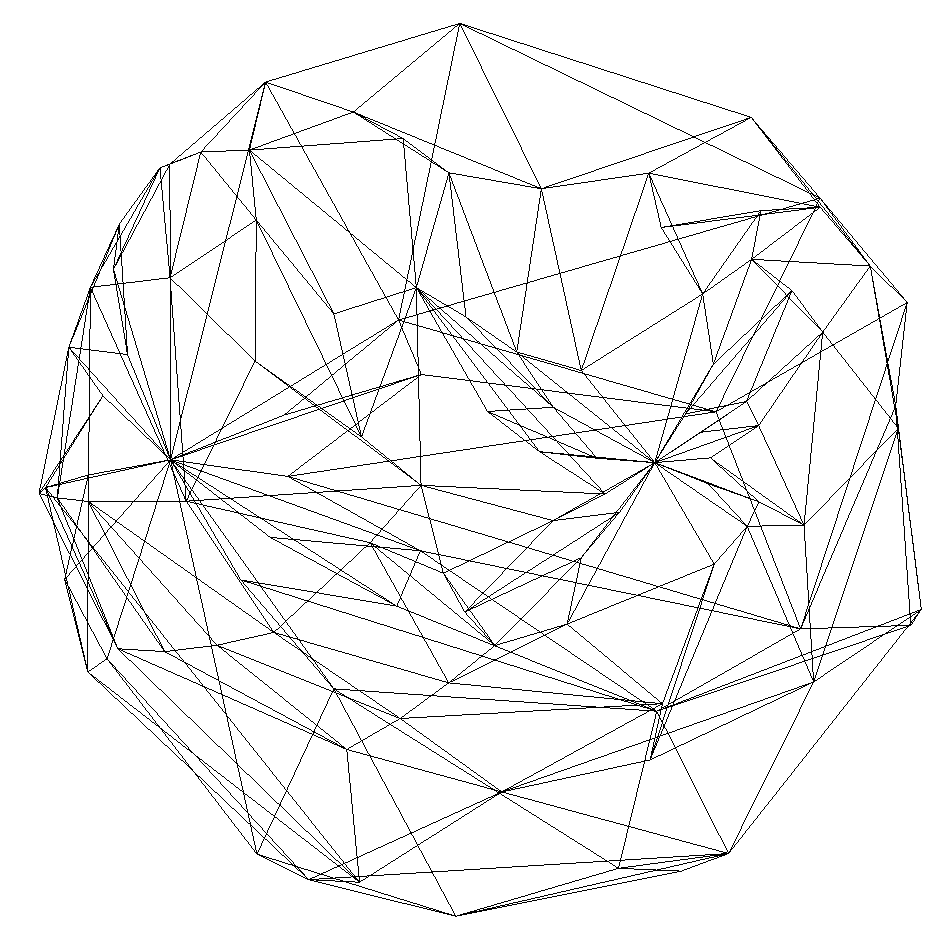
\includegraphics[scale=0.25]{imagenes/esfera_25.png} 
	\caption{Malla sphere.ply con una tasa de reducción del 25\%.} \label{fig:esfera_25.png}
\end{figure}

\subsection{Beethoven}
Cuando aplicamos las mismas tasas de reducción pero sobre una figura con un mayor número de elementos, obtenemos que la simplificación se realiza de manera más eficiente en cuanto a la similitud con la original. Puesto que al tener más zonas homogéneas esta figura la simplificación es más exacta.\\

\begin{figure} %con el [H] le obligamos a situar aquí la figura
	\centering
	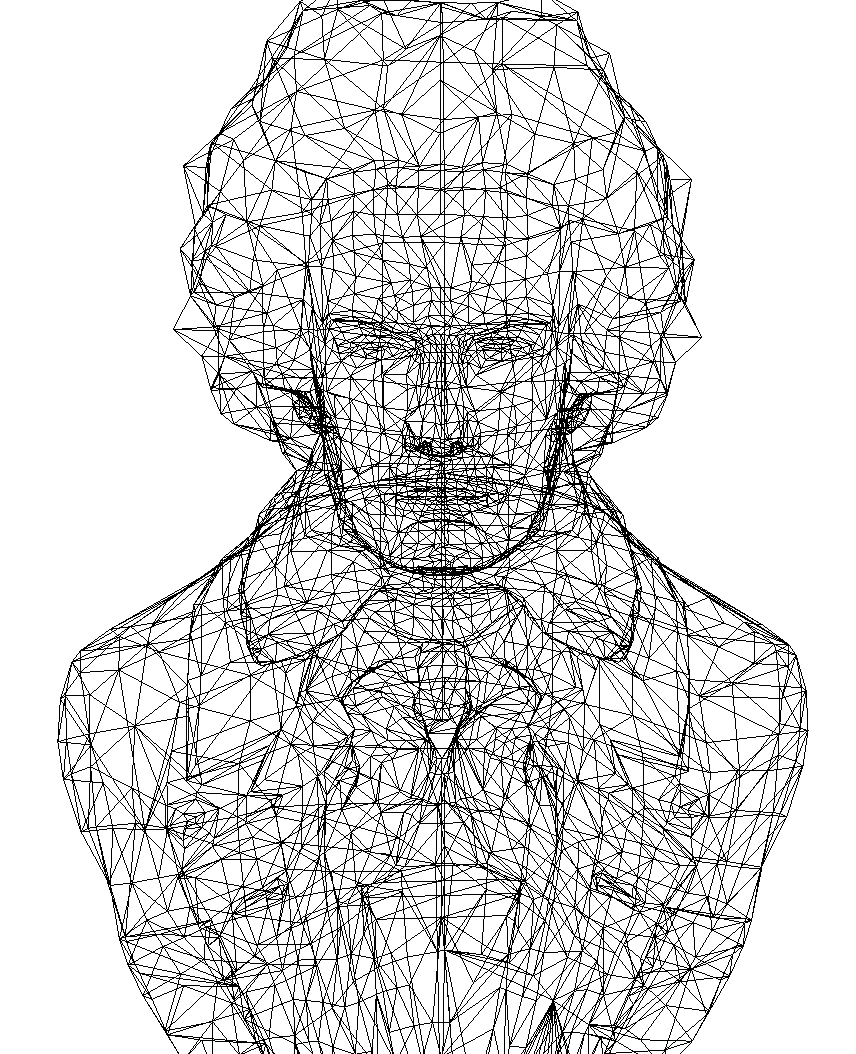
\includegraphics[scale=0.25]{imagenes/beethoven_90.png} 
	\caption{Malla beethoven.ply con una tasa de reducción del 90\%.} \label{fig:beethoven_90.png}
\end{figure}

En la primera simplificación, figura \ref{fig:beethoven_90.png} apenas notamos diferencia, al igual que en la esfera, una tasa de reducción alta consigue un resultado muy similar al original. Para ver los cambios tenemos que fijarnos en la parte baja de los hombros donde existe una zona de caras muy homogéneas y por tanto zonas más propensas a simplificarse.
\begin{figure} %con el [H] le obligamos a situar aquí la figura
	\centering
	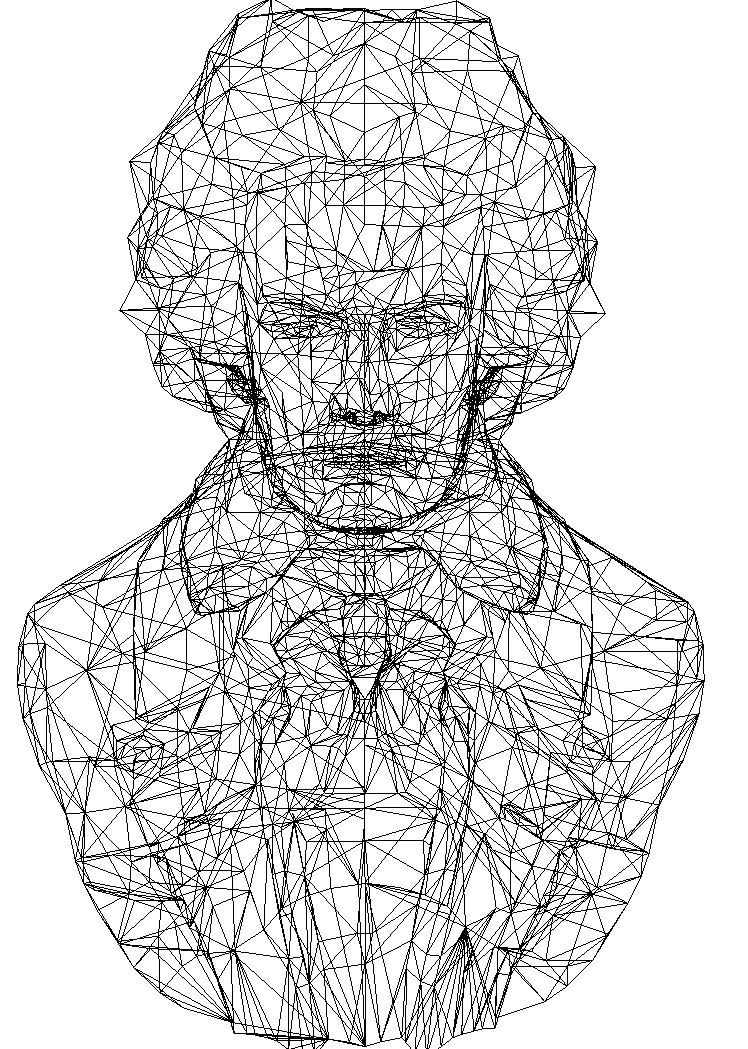
\includegraphics[scale=0.25]{imagenes/beethoven_75.png} 
	\caption{Malla beethoven.ply con una tasa de reducción del 75\%.} \label{fig:beethoven_75.png}
\end{figure}

Con la siguiente tasa de reducción al 75\%, figura \ref{fig:beethoven_75.png}, ya se empiezan a notar algunas partes menos definidas, pero solo apreciables si las comparamos con la original. Pero sigue manteniendo perfectamente la forma.\\
\begin{figure} %con el [H] le obligamos a situar aquí la figura
	\centering
	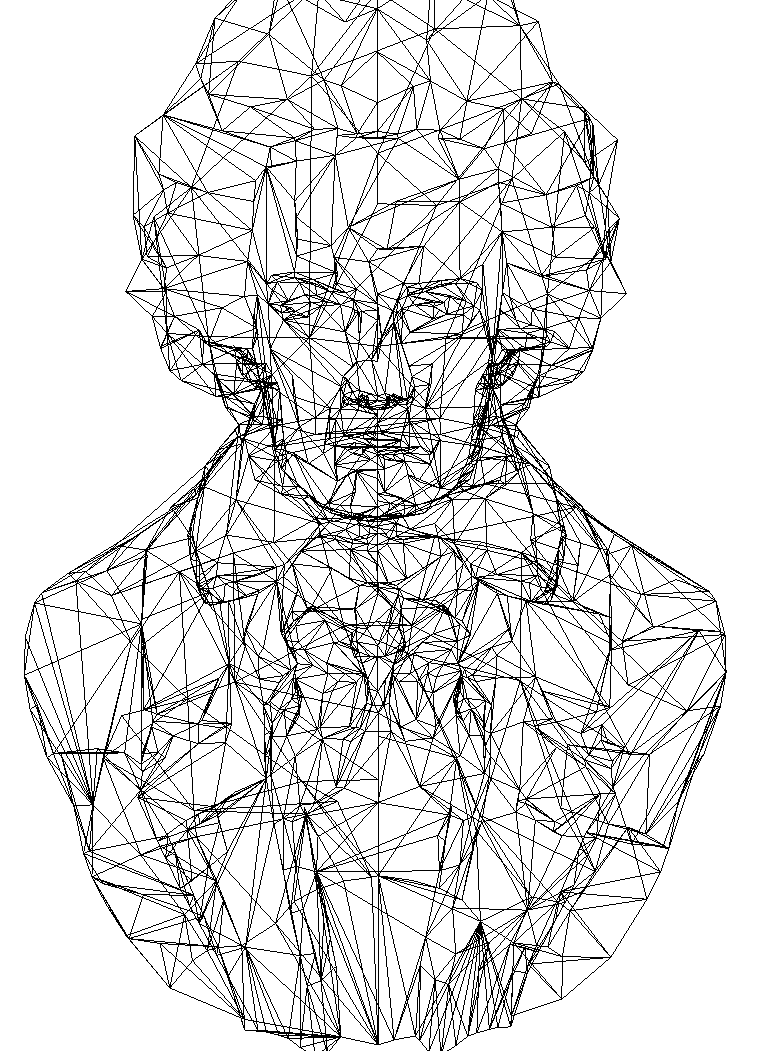
\includegraphics[scale=0.25]{imagenes/beethoven_50.png} 
	\caption{Malla beethoven.ply con una tasa de reducción del 50\%.} \label{fig:beethoven_50.png}
\end{figure}

Al aplicar la tasa de reducción al 50\%, figura \ref{fig:beethoven_50.png}, se produce un cambio significativo y ya se nota más la falta de calidad en la malla. Aunque sigue manteniendo la forma y se puede reconocer fácilmente la malla la cara ya no tiene la expresión original y muchos detalles se han perdido.\\

\begin{figure} %con el [H] le obligamos a situar aquí la figura
	\centering
	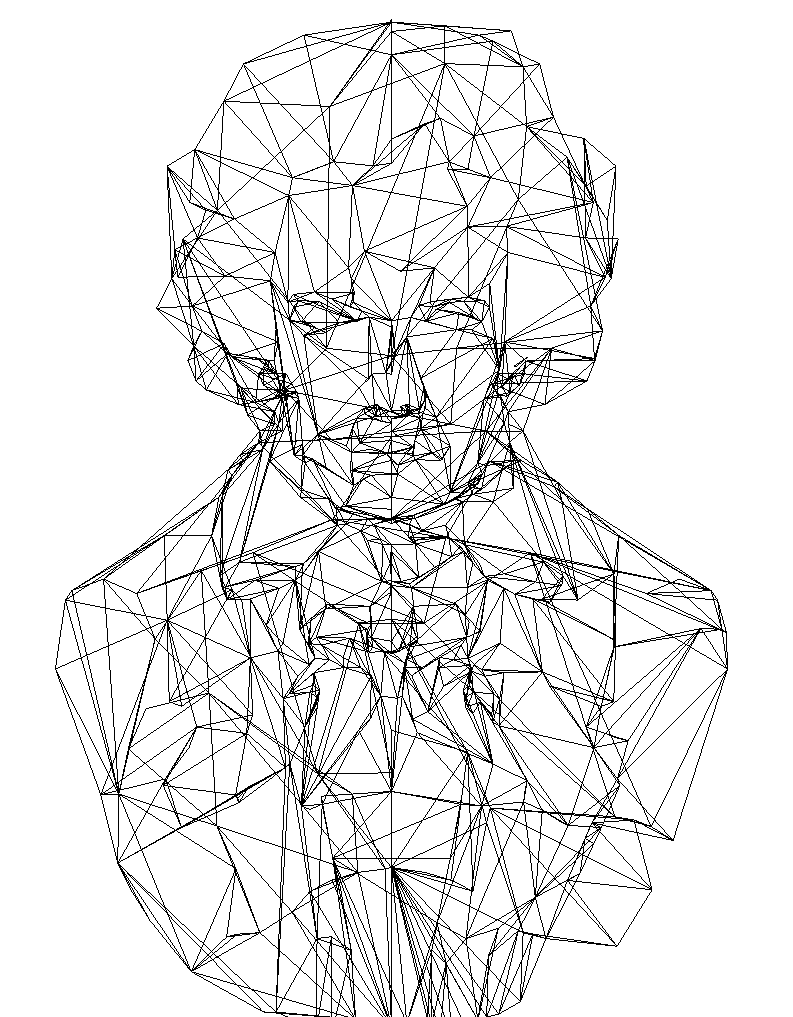
\includegraphics[scale=0.25]{imagenes/beethoven_25.png} 
	\caption{Malla beethoven.ply con una tasa de reducción del 25\%.} \label{fig:beethoven_25.png}
\end{figure}

Aplicando la última tasa de reducción al 25\%, figura \ref{fig:beethoven_25.png}, ya cuesta distinguir la figura y está muy poco definida.

\subsection{Big\_dodge}
Por último la malla con el mayor número de caras y con una característica más, que posee dos partes bien diferenciadas, una la carrocería del coche con superficies rectas y otra las ruedas y accesorios con una gran cantidad de ángulos y curvas. De está forma se podrá apreciar con más claridad la optimización del error conseguido en el método.\\

\begin{figure} %con el [H] le obligamos a situar aquí la figura
	\centering
	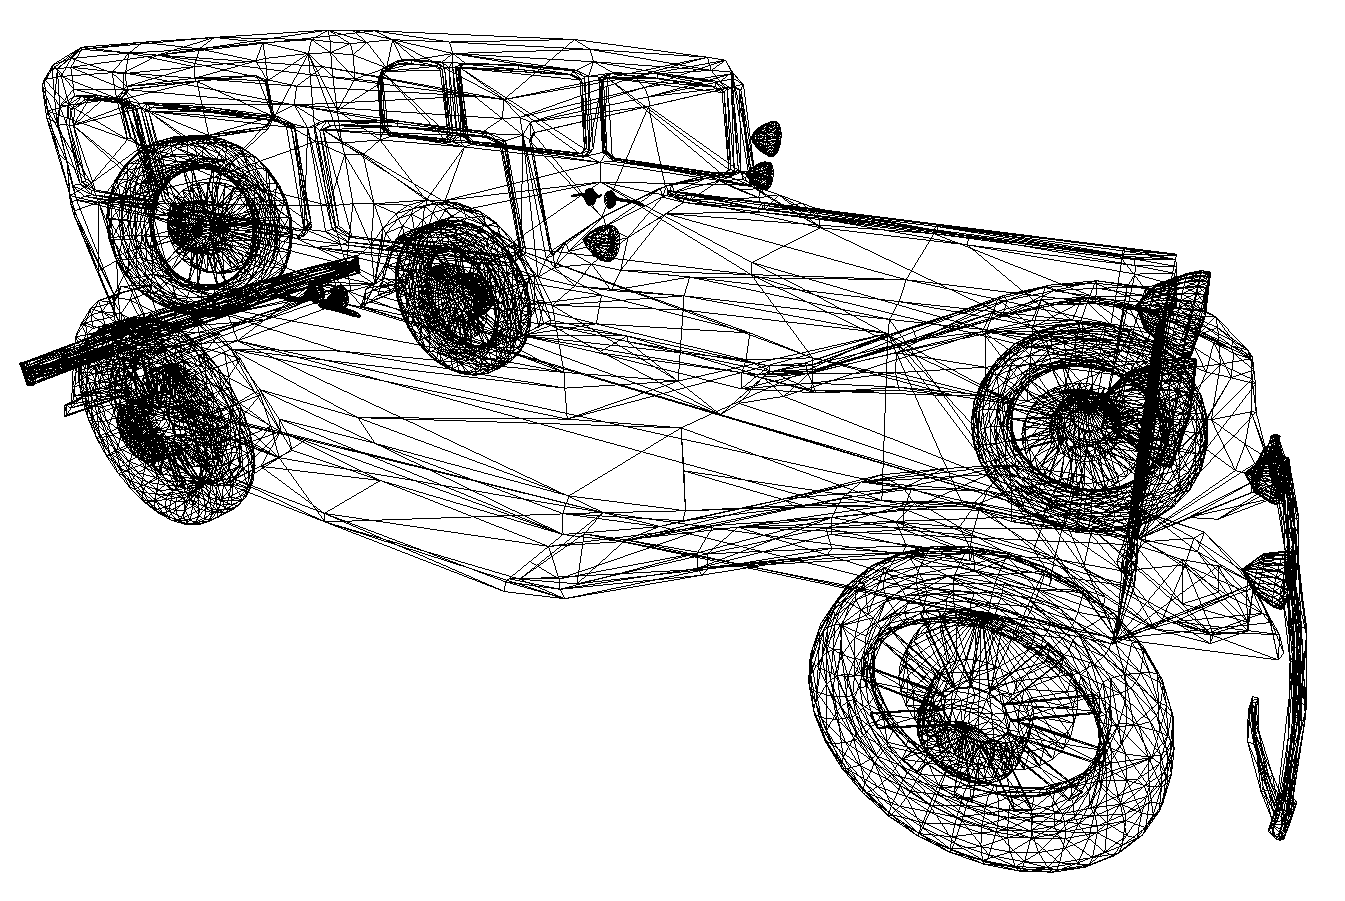
\includegraphics[scale=0.25]{imagenes/coche_90.png} 
	\caption{Malla big\_dodge.ply con una tasa de reducción del 90\%.} \label{fig:coche_90.png}
\end{figure}

En la primera simplificación, al 90\% figura \ref{fig:coche_90.png} los cambios son principalmente en la carrocería del coche donde los laterales ahora son caras más grandes y menos definidas. Se puede decir que el modelo no ha perdido a penas calidad.\\

\begin{figure} %con el [H] le obligamos a situar aquí la figura
	\centering
	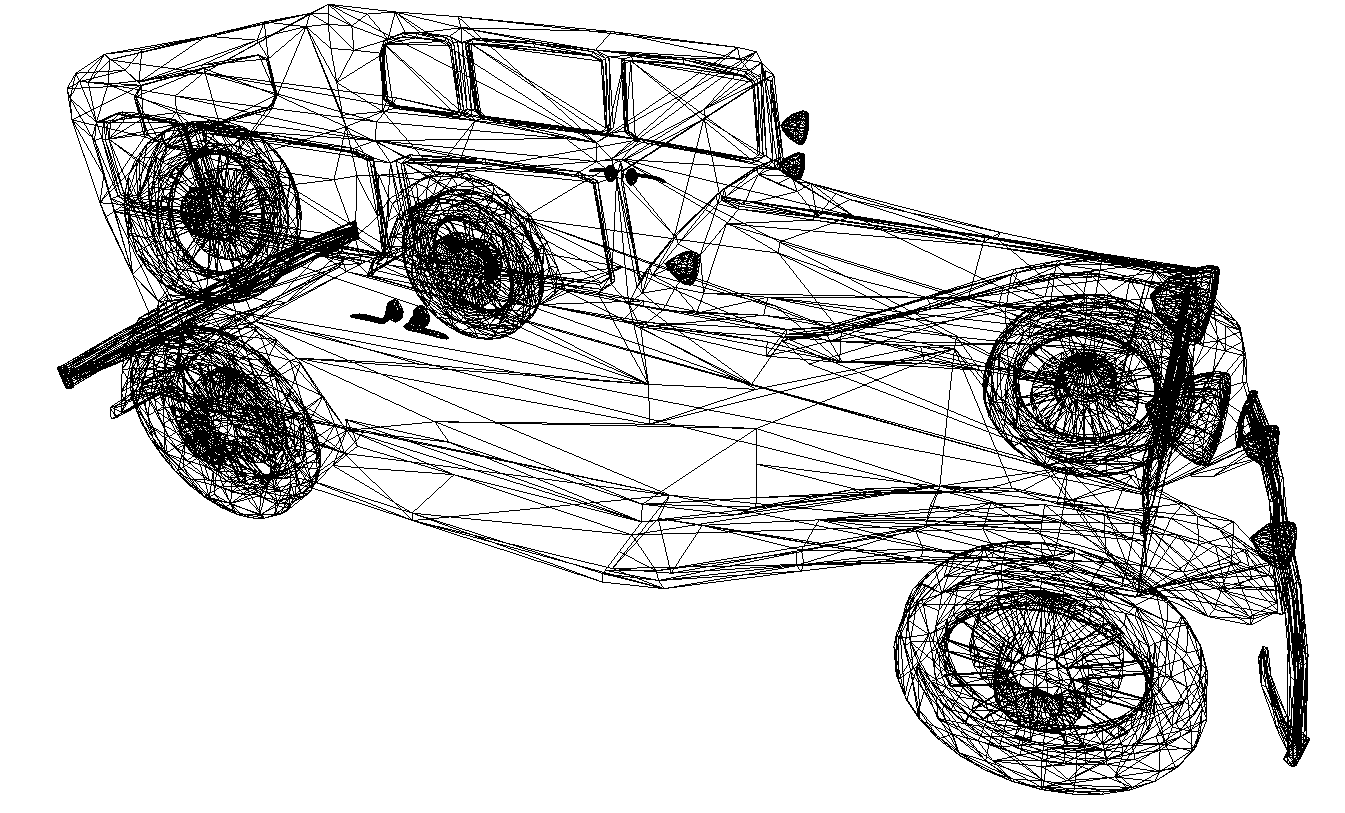
\includegraphics[scale=0.25]{imagenes/coche_75.png} 
	\caption{Malla big\_dodge.ply con una tasa de reducción del 75\%.} \label{fig:coche_75.png}
\end{figure}

En la segunda simplificación, al 75\% figura \ref{fig:coche_75.png}, los cambios en la carrocería son mayores y se empiezan a aplicar en las ruedas, en su lateral.\\

\begin{figure} %con el [H] le obligamos a situar aquí la figura
	\centering
	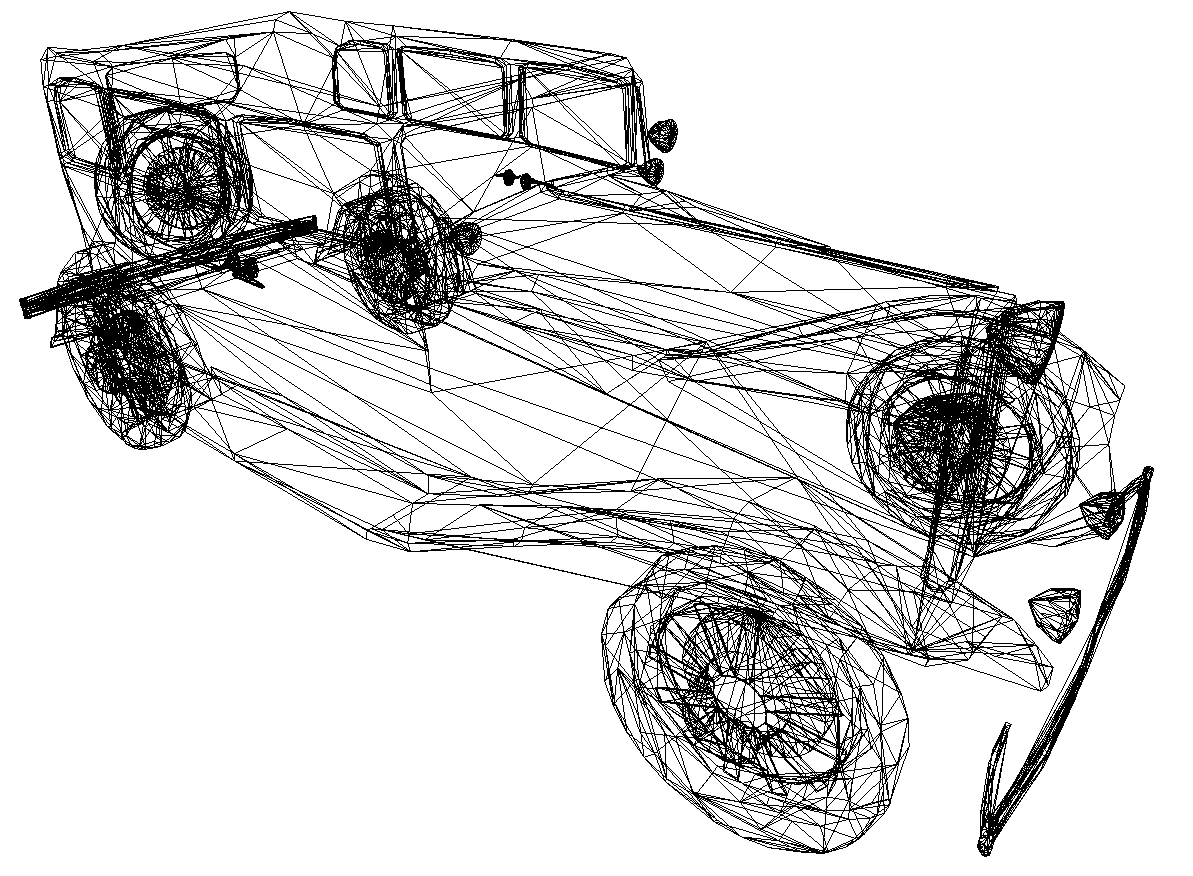
\includegraphics[scale=0.25]{imagenes/coche_50.png} 
	\caption{Malla big\_dodge.ply con una tasa de reducción del 50\%.} \label{fig:coche_50.png}
\end{figure}

Con la tercera simplificación, al 50\% figura \ref{fig:coche_50.png}, la forma se mantiene bastante bien y se ha concentrado la reducción en las ruedas y elementos algo más esféricos. Pero al igual que ocurría con Beethoven, el coche al tener muchos más elementos las simplificaciones permiten que se pueda simplificar más la malla sin perder mucha calidad.\\

\begin{figure} %con el [H] le obligamos a situar aquí la figura
	\centering
	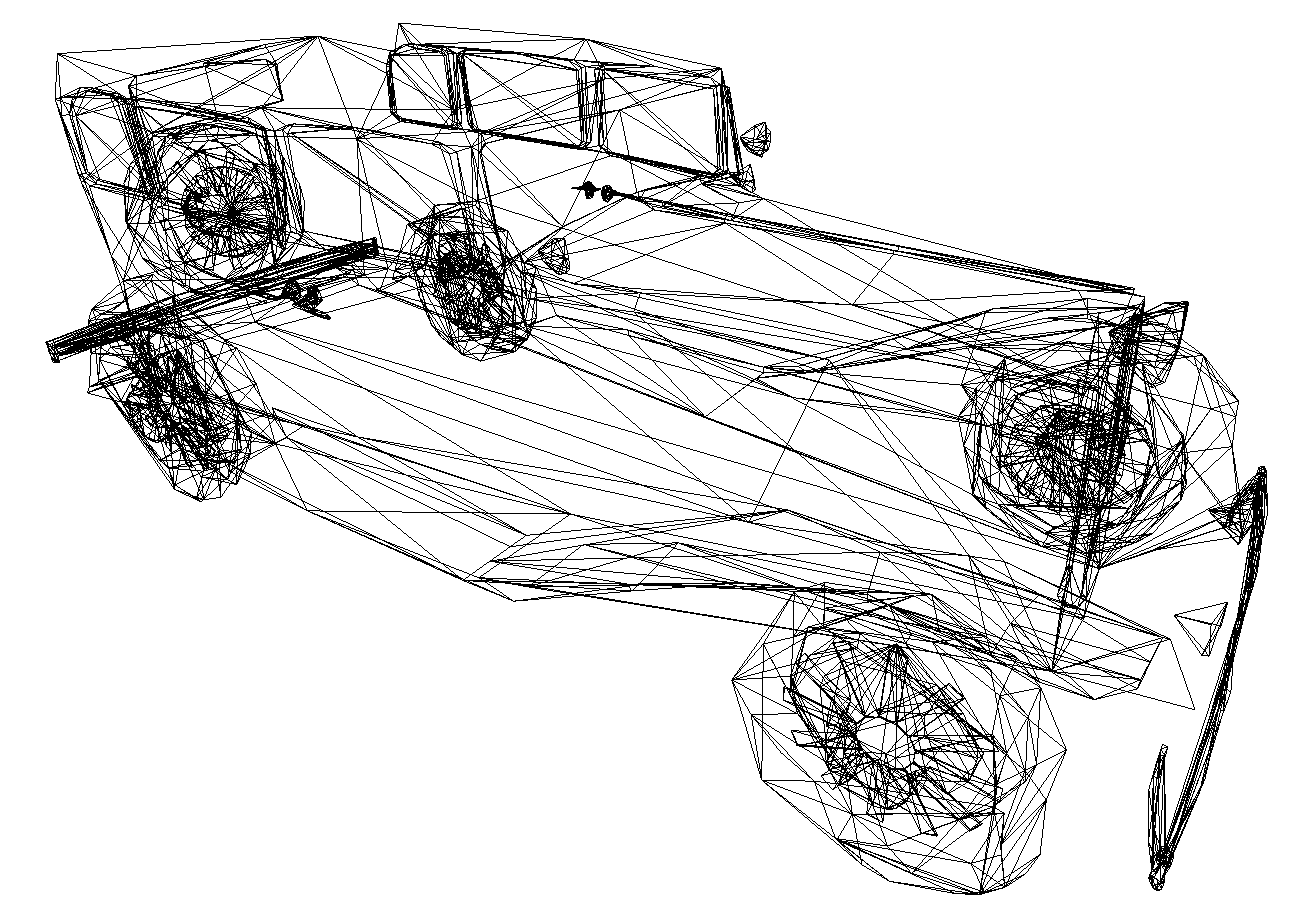
\includegraphics[scale=0.25]{imagenes/coche_25.png} 
	\caption{Malla big\_dodge.ply con una tasa de reducción del 25\%.} \label{fig:coche_25.png}
\end{figure}

En la cuarta y última simplificación, al 25\% figura \ref{fig:coche_25.png}, la estructura del coche ha quedado en grandes caras para cubrir la carrocería y los demás elementos se han simplificado en gran medida. Todavía se puede ver la forma de la malla original pero ya con mucha menos calidad.

\newpage
\subsection{Evaluación de las pruebas}
Como se comentó al principio del capítulo se han tomado los tiempos de ejecución del método \textit{decimation} al aplicarse cada una de las cuatro tasas de reducción y así poder comparar el costo en tiempo y el resultado obtenido, además para poder evaluar mejor el resultado se han obtenido el número de caras finales.\\

\begin{table}[]
	\centering
	\begin{tabular}{|l|l|l|l|}
		\hline
		\multicolumn{4}{|c|}{Tiempos de ejecución}     \\ \hline
		Reducción \% & big\_dodge & Bethoveen & sphere \\ \hline
		10           & 20,90      & 1,8       & 0,0423 \\ \hline
		25           & 46,80      & 3,68      & 0,0959 \\ \hline
		50           & 83,15      & 6,12      & 0,166  \\ \hline
		75           & 106,00     & 8,13      & 0,211  \\ \hline
	\end{tabular}
	\caption{Table de los tiempos de ejecución del método decimation sobre distintas mallas ply.}
	\label{tab:tiempos_decimation}
\end{table}

\begin{figure} %con el [H] le obligamos a situar aquí la figura
	\centering
	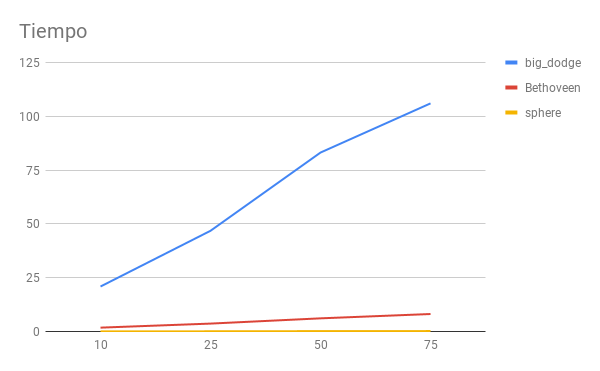
\includegraphics[scale=0.5]{imagenes/Tiempo.png} 
	\caption{Gráfica de la tabla \ref{tab:tiempos_decimation}, que muestra el aumento de costo al agrandar la tasas de } \label{fig:tiempo.png}
\end{figure}

En la tabla \ref{tab:tiempos_decimation} se puede observar como los tiempos de aplicación del método se incrementan en gran medida con forme aplicamos tasas de reducción más restrictivas. En la gráfica \ref{fig:tiempo.png} vemos como las mallas con menor número de elementos siguen un crecimiento moderado, mientras que la malla big\_dodge sigue un crecimiento prácticamente lineal. Esto es una relación directa entre el número de elementos a evaluar, pero recordemos que también se consigue una mayor calidad.\\

También hemos considerado el número de caras resultantes, que se puede observar en la tabla \ref{tab:caras} el número de caras es proporcional a la tasas de reducción. Esta relación se mantiene constante. Como el caso de las tasas al 90\% donde la calidad de la malla no se veía muy afectada y donde el número de caras es algo menor, esto es importante tenerlo en cuenta ya que para aplicar en un futuro la técnica de Level Of Details, todo lo que se pueda ahorrar en elementos sin comprometer mucho la calidad es una gran solución.

\begin{table}[]
	\centering
	\begin{tabular}{|r|c|c|c|}
		\hline
		\multicolumn{4}{|c|}{Número de Triángulos}                                                                                          \\ \hline
		\multicolumn{1}{|l|}{Reducción \%} & \multicolumn{1}{l|}{big\_dodge} & \multicolumn{1}{l|}{Bethoveen} & \multicolumn{1}{l|}{sphere} \\ \hline
		0                                  & 16.646                          & 5.030                          & 840                         \\ \hline
		10                                 & 14.982                          & 4.528                          & 756                         \\ \hline
		25                                 & 12.484                          & 3.772                          & 630                         \\ \hline
		50                                 & 8.324                           & 2.516                          & 420                         \\ \hline
		75                                 & 4.162                           & 1.258                          & 210                         \\ \hline
	\end{tabular}
	\caption{Tabla de número de caras sobre las mallas con distintos tipos de tasas de reducción}
	\label{tab:caras}
\end{table}

Por último es necesario analizar el tiempo entre figuras con respecto al número de caras de cada figura. En la tabla \ref{tab:inc_coche_beethoven}, tenemos en la segunda (Inc. Caras) columna el incremento de caras que existe entre la malla big\_dodge y Beethoven y en la tercera columna (Inc. Tiempo). La primera columna nos muestra que la proporción de caras es constante entre una malla y la otra, pero en la segunda columna nos indica que el factor tiempo crece cuanto mayor es la tasas de reducción. Si comparamos ambos resultados obtenemos la última columna (Diferencia) que indica la diferencia entre el aumento de caras y el aumento del tiempo, por tanto el factor tiempo crece mucho al aumentar el número de elementos a evaluar, crece por del orden de 9 veces por encima del aumento del número de caras.

\begin{table}[]
	\centering
\begin{tabular}{l|c|c|c|}
	\cline{2-4}
	Reducción \% & Inc. Caras  & \multicolumn{1}{l|}{Inc. Tiempo} & \multicolumn{1}{l|}{Diferencia} \\ \cline{2-4} 
	10           & 3,309343936 & 11,61111111                      & 8,301767175                     \\ \cline{2-4} 
	25           & 3,308745583 & 12,7173913                       & 9,408645721                     \\ \cline{2-4} 
	50           & 3,309650053 & 13,58660131                      & 10,27695125                     \\ \cline{2-4} 
	75           & 3,308426073 & 13,03813038                      & 9,729704308                     \\ \cline{2-4} 
\end{tabular}
	\caption{Tabla de diferencia entre el incremento de tiempo y el incremento de caras entre la malla de Big\_dodge y Beethoven.}
	\label{tab:inc_coche_beethoven}
\end{table}
%
\chapter{ Conclusiones}

\section{ Conclusiones}

Partiendo de los datos arrojados en las pruebas se puede concluir que el método de decimation junto con todos los demás de los que hace uso funciona correctamente. Los datos obtenidos son los esperados por el estudio de los algoritmos y la documentación leída. Para la malla resultante del método hay dos factores que definen como va a ser el resultado.

El primero es el número de elementos, pues cuantos más elementos más opciones de simplificación se podrán realizar afectando menos a la calidad resultante.

El segundo factor es la propia definición de la malla, si la malla posee grandes superficies compuestas por muchos elementos en el mismo plano o en planos muy próximos las simplificaciones se van a centrar en esa parte. Consiguiendo así que se reduzca el número de elementos sin modificar la forma de la malla.\\

Otro factor del proyecto ha sido el estudio de los algoritmos de procesamiento geométrico de simplificación, son algoritmos muy potentes basados en ideas sencillas. Pero que para nada son triviales de implementar, requieren unas condiciones muy específicas para funcionar correctamente y ahí radica su complejidad en modificar la malla manteniendo las propiedades y condiciones deseadas.\\

En cuanto a la estructura de datos de semi-aristas aladas es un concepto que la primera vez te choca, pero una buena implementación hace que el resto de la programación de algoritmos sea mucho más fácil y precisa. Accediendo a los elementos vecinos con suma rapidez y aprovechando el espacio en memoria.\\

Por parte de la API gráfica, OpenGL ha sido muy satisfactorio trabajar con ella puesto que provee una gran cantidad de funcionalidad para que el programador sea capaz de montar estructuras en memoria según sus necesidades. La forma de manipular la geometría y vista de los Shaders ha sido muy instructiva. Y por último la implementación de un sistema completo y utilizando las tecnologías actuales ha sido muy enriquecedor.\\


%
\chapter{ Trabajos Futuros}

En este capitulo se detallan posibles continuaciones del sistema desarrollado.

\section{ Trabajos Futuros}

Las mejoras que permite el sistema son muy amplias, al estar diseñado dentro de un área tan grande como es la informática gráfica se pueden realizar las siguientes mejoras: 

\begin{itemize}
	\item Mejorar la interfaz de usuario, permitiendo que se muestren datos de tiempo y número de elementos mediante mensajes.
	\item Se puede mejorar las opciones de visualización de la malla renderizada mediante una gestión de los buffers para que muestre la figura no solo en alambre o solido si no una combinación de ambas y un mapa de colores del error de borrar una semi-arista.
	\item Añadir otros algoritmos de procesado geométrico.
	\item Obtener la malla generada en formato .ply para guardarla en un fichero local.
\end{itemize}

En resumen, una vez tenemos un renderizador y una estructura optimizada para el procesado geométrico de mallas de triángulos, cualquier algoritmo que se desee implementar es posible, solo hay que añadirlo al sistema y generar la nueva malla o modificar la existente. 
%
%
%%\nocite{*}
\chapter*{}
\bibliography{Bibliografia}
\addcontentsline{toc}{chapter}{Bibliografía}
\label{bibliografia}
\bibliographystyle{plain}
%\bibliographystyle{miunsrturl}
%
\appendix
%\input{apendices/manual_usuario/manual_usuario}
\chapter{ Anexos}



\section{ Repositorio}

Todo el proyecto incluida la memoria e imagenes está subida a un repositorio público de github. En enlace es el siguiente:\\ \href{https://github.com/Joselmo/TFG_Modelator_Geometry_Processing}{https://github.com/Joselmo/TFG\_Modelator\_Geometry\_Processing}.

%\input{glosario/entradas_glosario}
% \addcontentsline{toc}{chapter}{Glosario}
% \printglossary
\chapter*{}
\thispagestyle{empty}

\end{document}
